% Options for packages loaded elsewhere
% Options for packages loaded elsewhere
\PassOptionsToPackage{unicode}{hyperref}
\PassOptionsToPackage{hyphens}{url}
\PassOptionsToPackage{dvipsnames,svgnames,x11names}{xcolor}
%
\documentclass[
  brazilian,
  letterpaper,
  DIV=11,
  numbers=noendperiod]{scrreprt}
\usepackage{xcolor}
\usepackage{amsmath,amssymb}
\setcounter{secnumdepth}{5}
\usepackage{iftex}
\ifPDFTeX
  \usepackage[T1]{fontenc}
  \usepackage[utf8]{inputenc}
  \usepackage{textcomp} % provide euro and other symbols
\else % if luatex or xetex
  \usepackage{unicode-math} % this also loads fontspec
  \defaultfontfeatures{Scale=MatchLowercase}
  \defaultfontfeatures[\rmfamily]{Ligatures=TeX,Scale=1}
\fi
\usepackage{lmodern}
\ifPDFTeX\else
  % xetex/luatex font selection
\fi
% Use upquote if available, for straight quotes in verbatim environments
\IfFileExists{upquote.sty}{\usepackage{upquote}}{}
\IfFileExists{microtype.sty}{% use microtype if available
  \usepackage[]{microtype}
  \UseMicrotypeSet[protrusion]{basicmath} % disable protrusion for tt fonts
}{}
\makeatletter
\@ifundefined{KOMAClassName}{% if non-KOMA class
  \IfFileExists{parskip.sty}{%
    \usepackage{parskip}
  }{% else
    \setlength{\parindent}{0pt}
    \setlength{\parskip}{6pt plus 2pt minus 1pt}}
}{% if KOMA class
  \KOMAoptions{parskip=half}}
\makeatother
% Make \paragraph and \subparagraph free-standing
\makeatletter
\ifx\paragraph\undefined\else
  \let\oldparagraph\paragraph
  \renewcommand{\paragraph}{
    \@ifstar
      \xxxParagraphStar
      \xxxParagraphNoStar
  }
  \newcommand{\xxxParagraphStar}[1]{\oldparagraph*{#1}\mbox{}}
  \newcommand{\xxxParagraphNoStar}[1]{\oldparagraph{#1}\mbox{}}
\fi
\ifx\subparagraph\undefined\else
  \let\oldsubparagraph\subparagraph
  \renewcommand{\subparagraph}{
    \@ifstar
      \xxxSubParagraphStar
      \xxxSubParagraphNoStar
  }
  \newcommand{\xxxSubParagraphStar}[1]{\oldsubparagraph*{#1}\mbox{}}
  \newcommand{\xxxSubParagraphNoStar}[1]{\oldsubparagraph{#1}\mbox{}}
\fi
\makeatother

\usepackage{color}
\usepackage{fancyvrb}
\newcommand{\VerbBar}{|}
\newcommand{\VERB}{\Verb[commandchars=\\\{\}]}
\DefineVerbatimEnvironment{Highlighting}{Verbatim}{commandchars=\\\{\}}
% Add ',fontsize=\small' for more characters per line
\usepackage{framed}
\definecolor{shadecolor}{RGB}{241,243,245}
\newenvironment{Shaded}{\begin{snugshade}}{\end{snugshade}}
\newcommand{\AlertTok}[1]{\textcolor[rgb]{0.68,0.00,0.00}{#1}}
\newcommand{\AnnotationTok}[1]{\textcolor[rgb]{0.37,0.37,0.37}{#1}}
\newcommand{\AttributeTok}[1]{\textcolor[rgb]{0.40,0.45,0.13}{#1}}
\newcommand{\BaseNTok}[1]{\textcolor[rgb]{0.68,0.00,0.00}{#1}}
\newcommand{\BuiltInTok}[1]{\textcolor[rgb]{0.00,0.23,0.31}{#1}}
\newcommand{\CharTok}[1]{\textcolor[rgb]{0.13,0.47,0.30}{#1}}
\newcommand{\CommentTok}[1]{\textcolor[rgb]{0.37,0.37,0.37}{#1}}
\newcommand{\CommentVarTok}[1]{\textcolor[rgb]{0.37,0.37,0.37}{\textit{#1}}}
\newcommand{\ConstantTok}[1]{\textcolor[rgb]{0.56,0.35,0.01}{#1}}
\newcommand{\ControlFlowTok}[1]{\textcolor[rgb]{0.00,0.23,0.31}{\textbf{#1}}}
\newcommand{\DataTypeTok}[1]{\textcolor[rgb]{0.68,0.00,0.00}{#1}}
\newcommand{\DecValTok}[1]{\textcolor[rgb]{0.68,0.00,0.00}{#1}}
\newcommand{\DocumentationTok}[1]{\textcolor[rgb]{0.37,0.37,0.37}{\textit{#1}}}
\newcommand{\ErrorTok}[1]{\textcolor[rgb]{0.68,0.00,0.00}{#1}}
\newcommand{\ExtensionTok}[1]{\textcolor[rgb]{0.00,0.23,0.31}{#1}}
\newcommand{\FloatTok}[1]{\textcolor[rgb]{0.68,0.00,0.00}{#1}}
\newcommand{\FunctionTok}[1]{\textcolor[rgb]{0.28,0.35,0.67}{#1}}
\newcommand{\ImportTok}[1]{\textcolor[rgb]{0.00,0.46,0.62}{#1}}
\newcommand{\InformationTok}[1]{\textcolor[rgb]{0.37,0.37,0.37}{#1}}
\newcommand{\KeywordTok}[1]{\textcolor[rgb]{0.00,0.23,0.31}{\textbf{#1}}}
\newcommand{\NormalTok}[1]{\textcolor[rgb]{0.00,0.23,0.31}{#1}}
\newcommand{\OperatorTok}[1]{\textcolor[rgb]{0.37,0.37,0.37}{#1}}
\newcommand{\OtherTok}[1]{\textcolor[rgb]{0.00,0.23,0.31}{#1}}
\newcommand{\PreprocessorTok}[1]{\textcolor[rgb]{0.68,0.00,0.00}{#1}}
\newcommand{\RegionMarkerTok}[1]{\textcolor[rgb]{0.00,0.23,0.31}{#1}}
\newcommand{\SpecialCharTok}[1]{\textcolor[rgb]{0.37,0.37,0.37}{#1}}
\newcommand{\SpecialStringTok}[1]{\textcolor[rgb]{0.13,0.47,0.30}{#1}}
\newcommand{\StringTok}[1]{\textcolor[rgb]{0.13,0.47,0.30}{#1}}
\newcommand{\VariableTok}[1]{\textcolor[rgb]{0.07,0.07,0.07}{#1}}
\newcommand{\VerbatimStringTok}[1]{\textcolor[rgb]{0.13,0.47,0.30}{#1}}
\newcommand{\WarningTok}[1]{\textcolor[rgb]{0.37,0.37,0.37}{\textit{#1}}}

\usepackage{longtable,booktabs,array}
\newcounter{none} % for unnumbered tables
\usepackage{calc} % for calculating minipage widths
% Correct order of tables after \paragraph or \subparagraph
\usepackage{etoolbox}
\makeatletter
\patchcmd\longtable{\par}{\if@noskipsec\mbox{}\fi\par}{}{}
\makeatother
% Allow footnotes in longtable head/foot
\IfFileExists{footnotehyper.sty}{\usepackage{footnotehyper}}{\usepackage{footnote}}
\makesavenoteenv{longtable}
\usepackage{graphicx}
\makeatletter
\newsavebox\pandoc@box
\newcommand*\pandocbounded[1]{% scales image to fit in text height/width
  \sbox\pandoc@box{#1}%
  \Gscale@div\@tempa{\textheight}{\dimexpr\ht\pandoc@box+\dp\pandoc@box\relax}%
  \Gscale@div\@tempb{\linewidth}{\wd\pandoc@box}%
  \ifdim\@tempb\p@<\@tempa\p@\let\@tempa\@tempb\fi% select the smaller of both
  \ifdim\@tempa\p@<\p@\scalebox{\@tempa}{\usebox\pandoc@box}%
  \else\usebox{\pandoc@box}%
  \fi%
}
% Set default figure placement to htbp
\def\fps@figure{htbp}
\makeatother



\ifLuaTeX
\usepackage[bidi=basic,shorthands=off]{babel}
\else
\usepackage[bidi=default,shorthands=off]{babel}
\fi
\ifLuaTeX
  \usepackage{selnolig} % disable illegal ligatures
\fi


\setlength{\emergencystretch}{3em} % prevent overfull lines

\providecommand{\tightlist}{%
  \setlength{\itemsep}{0pt}\setlength{\parskip}{0pt}}



 


\KOMAoption{captions}{tableheading}
\makeatletter
\@ifpackageloaded{tcolorbox}{}{\usepackage[skins,breakable]{tcolorbox}}
\@ifpackageloaded{fontawesome5}{}{\usepackage{fontawesome5}}
\definecolor{quarto-callout-color}{HTML}{909090}
\definecolor{quarto-callout-note-color}{HTML}{0758E5}
\definecolor{quarto-callout-important-color}{HTML}{CC1914}
\definecolor{quarto-callout-warning-color}{HTML}{EB9113}
\definecolor{quarto-callout-tip-color}{HTML}{00A047}
\definecolor{quarto-callout-caution-color}{HTML}{FC5300}
\definecolor{quarto-callout-color-frame}{HTML}{acacac}
\definecolor{quarto-callout-note-color-frame}{HTML}{4582ec}
\definecolor{quarto-callout-important-color-frame}{HTML}{d9534f}
\definecolor{quarto-callout-warning-color-frame}{HTML}{f0ad4e}
\definecolor{quarto-callout-tip-color-frame}{HTML}{02b875}
\definecolor{quarto-callout-caution-color-frame}{HTML}{fd7e14}
\makeatother
\makeatletter
\@ifpackageloaded{bookmark}{}{\usepackage{bookmark}}
\makeatother
\makeatletter
\@ifpackageloaded{caption}{}{\usepackage{caption}}
\AtBeginDocument{%
\ifdefined\contentsname
  \renewcommand*\contentsname{Índice}
\else
  \newcommand\contentsname{Índice}
\fi
\ifdefined\listfigurename
  \renewcommand*\listfigurename{Lista de Figuras}
\else
  \newcommand\listfigurename{Lista de Figuras}
\fi
\ifdefined\listtablename
  \renewcommand*\listtablename{Lista de Tabelas}
\else
  \newcommand\listtablename{Lista de Tabelas}
\fi
\ifdefined\figurename
  \renewcommand*\figurename{Figura}
\else
  \newcommand\figurename{Figura}
\fi
\ifdefined\tablename
  \renewcommand*\tablename{Tabela}
\else
  \newcommand\tablename{Tabela}
\fi
}
\@ifpackageloaded{float}{}{\usepackage{float}}
\floatstyle{ruled}
\@ifundefined{c@chapter}{\newfloat{codelisting}{h}{lop}}{\newfloat{codelisting}{h}{lop}[chapter]}
\floatname{codelisting}{Listagem}
\newcommand*\listoflistings{\listof{codelisting}{Lista de Listagens}}
\makeatother
\makeatletter
\makeatother
\makeatletter
\@ifpackageloaded{caption}{}{\usepackage{caption}}
\@ifpackageloaded{subcaption}{}{\usepackage{subcaption}}
\makeatother
\usepackage{bookmark}
\IfFileExists{xurl.sty}{\usepackage{xurl}}{} % add URL line breaks if available
\urlstyle{same}
\hypersetup{
  pdftitle={Apostila de Crescimento},
  pdfauthor={Caio Vilella},
  pdflang={pt-BR},
  colorlinks=true,
  linkcolor={blue},
  filecolor={Maroon},
  citecolor={Blue},
  urlcolor={Blue},
  pdfcreator={LaTeX via pandoc}}


\title{Apostila de Crescimento}
\author{Caio Vilella}
\date{}
\begin{document}
\maketitle

\renewcommand*\contentsname{Índice}
{
\setcounter{tocdepth}{2}
\tableofcontents
}

\bookmarksetup{startatroot}

\chapter*{Preface}\label{preface}
\addcontentsline{toc}{chapter}{Preface}

\markboth{Preface}{Preface}

This is a Quarto book.

To learn more about Quarto books visit
\url{https://quarto.org/docs/books}.

\begin{Shaded}
\begin{Highlighting}[]
\DecValTok{1} \SpecialCharTok{+} \DecValTok{1}
\end{Highlighting}
\end{Shaded}

\begin{verbatim}
[1] 2
\end{verbatim}

\bookmarksetup{startatroot}

\chapter{A Contabilidade do Crescimento e a Distribuição de
Renda}\label{sec-contabilidade}

\section{Introdução}\label{introduuxe7uxe3o}

O debate sobre o \textbf{crescimento econômico} e a \textbf{distribuição
de renda} tem sido central na economia, ganhando renovada atenção,
especialmente após eventos como a Grande Recessão de 2008-09. A questão
fundamental que permeia este campo de estudo é: os resultados dos
modelos de determinação da renda de curto prazo podem ser extrapolados
para o longo prazo? E, mais crucialmente, o que explica o diferencial de
renda entre os países e como a distribuição da renda afeta a dinâmica do
crescimento?

Este capítulo explora a \textbf{contabilidade do crescimento} sob a
ótica da distribuição de renda, contrastando as abordagens neoclássica e
heterodoxa. Nosso objetivo é compreender como a forma pela qual o
excedente gerado na economia é distribuído entre capital e trabalho
influencia a acumulação e o ritmo de expansão econômica. Aprofundaremos
nas diferentes perspectivas teóricas, desde os clássicos até os modelos
pós-keynesianos de segunda geração, que servem de base para os modelos
de crescimento liderados pela demanda.

\section{A Distribuição da Renda: Conceitos
Fundamentais}\label{a-distribuiuxe7uxe3o-da-renda-conceitos-fundamentais}

Para entender a relação entre distribuição e crescimento, é essencial
distinguir os diferentes níveis de análise da distribuição de renda:

\begin{itemize}
\item
  \textbf{Distribuição Primária da Renda:} Refere-se à forma como a
  riqueza é inicialmente apropriada pelos fatores de produção (capital e
  trabalho) no processo produtivo. É a divisão do produto social entre
  lucros e salários, determinada pelas forças de mercado e pelas
  relações de poder. Em termos simples, quem se apropria do excedente
  gerado? Se considerarmos a renda total (\(Y\)) como a soma dos lucros
  (\(\Pi\)) e dos salários (\(W\)), temos \(Y = \Pi + W\). Dividindo por
  \(Y\), obtemos a participação de cada fator na renda:
  \(\frac{\Pi}{Y} + \frac{W}{Y} = 1\).
\item
  \textbf{Distribuição Secundária da Renda:} Diz respeito à
  redistribuição da renda disponível após a intervenção do Estado, por
  meio de políticas fiscais (impostos) e sociais (transferências e
  benefícios). Esta etapa afeta a distribuição entre classes sociais e
  indivíduos, moldando a renda disponível para consumo e poupança.
\end{itemize}

A forma como a distribuição de renda é tratada varia significativamente
entre as diferentes escolas de pensamento econômico. Essa distinção é
crucial para entender as implicações sobre o crescimento.

\subsection{A Visão Neoclássica}\label{a-visuxe3o-neocluxe1ssica}

Na abordagem neoclássica, a distribuição de renda é determinada pela
\textbf{contribuição relativa de cada fator de produção} para a produção
agregada, mediada pelos seus preços relativos. A produtividade marginal
dos fatores (capital e trabalho) define suas remunerações.

Consideremos \(L\) como sendo a quantidade de trabalho e \(K\) a
quantidade física de capital. O sobrescrito \(D\) representa a variável
de demanda, enquanto o sobrescrito \(S\),a de oferta. Por exemplo:
\(L^D\) seria a quanitdade demandada de trabalho e assim por diante.
Além disso, vamos representar a taxa de lucro por \(r\) e a a taxa de
salários reais por \(w\). Se a oferta deve equivaler a demanda no estado
estacionário então teremos que:

\[
\begin{aligned}
rK^S + wL^S = rK^D + w L^D\\
r (K^S - K^D) = w (L^D - L^S)\\
\frac{r}{w} = \frac{L^D - L^S}{K^S - K^D}
\end{aligned}
\]

Em um mercado competitivo, a taxa de lucro (preço do capital) e o
salário (preço do trabalho) se ajustam para igualar a oferta e a demanda
por esses fatores. A ideia central é que, se a demanda por trabalho
aumentar, deveria haver algum mecanismo (a substituição de trabalho por
capital) para levar à queda do salário em relação ao lucro para
reequilibrar o mercado. Da mesma forma, se o capital se torna abundante,
sua taxa de retorno (lucro) deveria cair em relação ao salário.

Nesses modelos, o crescimento econômico é frequentemente explicado por
fatores exógenos, como o progresso tecnológico e o crescimento
populacional. A poupança, embora importante para o nível de capital, não
teria um impacto duradouro sobre a taxa de crescimento de \emph{steady
state} em modelos mais antigos. Versões mais recentes, como a teoria do
crescimento endógeno, incorporam o capital humano e a inovação,
permitindo que a poupança e o investimento tenham um efeito mais direto
na taxa de crescimento de longo prazo, mas a distribuição de renda ainda
é vista como um resultado da tecnologia e das preferências, e não como
um determinante ativo do crescimento.

\subsection{A Visão Heterodoxa e
Pós-Keynesiana}\label{a-visuxe3o-heterodoxa-e-puxf3s-keynesiana}

Em contraste, a teoria de crescimento heterodoxa, e em particular a
tradição pós-keynesiana, resgata o \textbf{elo causal entre distribuição
e crescimento}. Nesta abordagem, a distribuição da renda não é um mero
resultado da tecnologia ou da escassez relativa dos fatores, mas sim um
fator ativo que influencia a taxa de crescimento da economia. O fato de
os preços relativos não determinarem unicamente a distribuição de renda
confere maior liberdade aos modelos pós-keynesianos, permitindo que a
\textbf{luta de classes} e as relações de poder desempenhem um papel
predominante na determinação da distribuição.

Autores clássicos como David Ricardo e Karl Marx já abordavam a
distribuição de renda a partir de fatores socioinstitucionais. A
\textbf{lei de ferro dos salários} de Ricardo, por exemplo, postulava
que os salários tenderiam ao nível de subsistência do trabalhador,
deixando a taxa de lucro como um resíduo do excedente produzido. A
acumulação de capital (\(g\)) era então determinada pela propensão a
poupar dos capitalistas (\(s_\Pi\)) e pela taxa de lucro (\(r\)), ou
seja,
\begin{equation}\protect\phantomsection\label{eq-gs}{g_s = s_r r}\end{equation}

No entanto, essa visão ainda pressupunha a validade da Lei de Say, onde
a poupança se converteria automaticamente em investimento, explicando o
crescimento pelo lado da oferta.

Os clássicos também identificaram limites exógenos à acumulação: Ricardo
apontava para os rendimentos decrescentes do fator terra, enquanto Marx
elaborou a lei da tendência à queda da taxa de lucro devido ao aumento
da composição orgânica do capital. Ambos, de diferentes formas, buscavam
explicar o desemprego e os limites ao crescimento em pontos anteriores
ao pleno emprego.

A \textbf{primeira geração de modelos pós-keynesianos}, desenvolvida por
autores como Nicholas Kaldor e Joan Robinson, inverteu a causalidade
clássica. Baseando-se no Princípio da Demanda Efetiva de Keynes, eles
argumentaram que as decisões de investimento das firmas e a acumulação
de capital determinam a distribuição funcional da renda. A taxa de lucro
(\(r\)) passou a ser vista como dependente da taxa de acumulação (\(g\))
e da propensão a poupar dos capitalistas (\(s_r\)): \(r = g/s_r\).

Assim,a distribuição de renda é um \emph{resultado} da acumulação de
capital, e não uma pré-condição. Conforme muda a taxa de acumulação, a
distribuição de renda se altera e muda também a taxa de poupança.

A \textbf{segunda geração de modelos pós-keynesianos}, inspirada nos
trabalhos de Michal Kalecki e Josef Steindl, aprofundou essa
perspectiva. Nesses modelos, a taxa de lucro dos capitalistas (\(r\)) é
determinada pela \textbf{participação dos lucros na renda} (\(\pi\)),
pelo \textbf{grau de utilização da capacidade instalada} (\(u\)) e pela
\textbf{relação capital-produto} (\(v\)). A relação pode ser expressa
como:

\begin{equation}\protect\phantomsection\label{eq-r}{r = \frac{\pi u}{v}}\end{equation}

Nesta formulação, a \textbf{demanda agregada} passa a afetar a
lucratividade por meio do grau de utilização da capacidade. Isso
significa que variações na demanda podem levar a mudanças no grau de
utilização, que por sua vez impactam a taxa de lucro, mas não
necessariamente a distribuição de renda.

Essa é uma característica fundamental dos modelos de crescimento
liderados pela demanda, onde o \textbf{Princípio da Demanda Efetiva
permanece válido no longo prazo}. A distirbuição de renda é dada pelo
grau de competição dos mercados, mas mudanças no nível de demanda
agregada podem afetar a taxa de lucro do capital por meio do grau de
utilização.

\begin{tcolorbox}[enhanced jigsaw, arc=.35mm, bottomrule=.15mm, bottomtitle=1mm, breakable, colback=white, colbacktitle=quarto-callout-note-color!10!white, colframe=quarto-callout-note-color-frame, coltitle=black, left=2mm, leftrule=.75mm, opacityback=0, opacitybacktitle=0.6, rightrule=.15mm, title=\textcolor{quarto-callout-note-color}{\faInfo}\hspace{0.5em}{O Princípio da Demanda Efetiva no Longo Prazo}, titlerule=0mm, toprule=.15mm, toptitle=1mm]

Nos modelos pós-keynesianos de segunda geração, o Princípio da Demanda
Efetiva gera alguns resultados que serão ressaltados ao logno da
apostila:

\begin{itemize}
\tightlist
\item
  \textbf{Efeito multiplicador da renda:} Um aumento no investimento ou
  em outros componentes autônomos da demanda gera um aumento maior na
  renda.
\item
  \textbf{Investimento gera poupança:} Diferente da visão clássica, o
  investimento não é limitado pela poupança pré-existente; ele cria a
  poupança necessária para financiá-lo.
\item
  \textbf{Caráter dual do investimento:} O investimento não apenas
  adiciona à capacidade produtiva, mas também gera demanda.
\item
  \textbf{Oferta se ajusta à demanda:} A produção se ajusta para atender
  à demanda agregada, e não o contrário.
\end{itemize}

\end{tcolorbox}

\section{Contabilidade do Crescimento e Modelos Liderados pela
Demanda}\label{sec-contabildiade}

Na Teoria Geral do Emprego do Juro e da Moeda, Keynes (1926) assumiu que
o consumo seria uma função da renda \((C= cY)\) para garantir que
ajustes no nível da renda equilibraram o mercado de bens, pois:

\[
\begin{aligned}
Y= C+I\\
Y = cY+I \\
Y-cY=I \\
Y(1-c)=I\\
Y=\frac{I}{1-c}
\end{aligned}
\]

onde: \(Y\) é a renda; \(I\) é o investimento agregado; \(C\) é o
consumo agregado; \(c\) é a propensão marginal a consumir.

Em que a propensão a consumir seria uma parcela (uma porcentagem) da
renda. Isso quer dizer que se \(c=0,8\), a comunidade analisada
cosumiria 80\% de cada unidade monetária obtida de renda. Logo, podemos
ver que o denominador da renda de equilíbrio \((1-c)\) é a porcentagem
poupada \((1-0,8=0,2)\). Chamemos, portanto, \(s\) de a propensão a
poupar de determinada sociedade para expressar a equação do
\textbf{nível} da renda como:

\begin{equation}\protect\phantomsection\label{eq-Y}{Y=\frac{I}{s}}\end{equation}

Este é o \textbf{nível} de renda que equilibra o mercado de bens,
igualando o \textbf{nível} de poupança \((S)\) com o nível de
investimento \((I)\), isto é: \(I=S\). Agora vamos partir desta
identidade contábil e dividir os dois lados pelo estoque de capital para
ter uma representação dinâmica do modelo de Keynes:

\begin{equation}\protect\phantomsection\label{eq-IK}{
\frac{I}{K}=\frac{S}{K}
}\end{equation}

Eu me referi como ``dinâmica'' pelo fato de o lado esquerdo da equação
Equação~\ref{eq-IK} ser a taxa (porcentagem) de crescimento do estoque
de capital. Isso fica fácil de ver se você pensar no investimento como a
variação do estoque de capital e notar que \(\Delta K = I\); Portanto:
\(I/K = \Delta K / K = g_K\).

Agora vamos seguir esta análise assumindo que a poupança é determinada
pela propensão a poupar da renda (assim como Keynes fez em sua análise
estática):

\begin{equation}\protect\phantomsection\label{eq-gk-cont}{\begin{aligned}
\frac{I}{K} &= \frac{s Y}{K}\\
g_K &= s \frac{Y}{K}
\end{aligned}}\end{equation}

Este já poderia ser o nosso ``resutlado final'' algébrico, mas traria
pouca informação do ponto de vista econômico. Assim, vamos ter que fazer
algumas manipulações importantíssimas para entender a intuição
econômica.

Primeiro vamos multiplicar a Equação~\ref{eq-gk-cont} por 1. Mas não
qualquer ``1'', vamos escolher um número ``1'' especial, que apesar de
não mudar o resutlado matemático, trará intuição econômica para a
análise. Vamos chamar o produto máximo que a economia é capaz de
produzir de \(Y_K\) e então multiplicar a Equação~\ref{eq-gk-cont} por
\(Y_K / Y_K\):

\begin{equation}\protect\phantomsection\label{eq-gk-cont2}{
\begin{aligned}
g_K = s \frac{Y}{K} \frac{Y_K}{Y_K}\\
g_K = s \frac{Y}{Y_K} \frac{Y_K}{K}
\end{aligned}}\end{equation} Aqui precisamos ir com calma e entender
cada termo, propositalente escrito separado, desta equação.

Repare que \(\frac{Y}{Y_K}\) é a divisão do produto corrente (pense em
PIB se achar que facilita a intuição) pelo seu nível máximo. Se este
resultado for 80\%, por exemplo, significaria que a economia está
operando a 80\% de sua capacidade instalada. De agora em diante
chamaremos isso de \textbf{grau de utilização da capacidade Instalada}
representado pela letra \(u\).

O termo seguinte vamos ler de cabeça para baixo: \(\frac{K}{Y_K}\). Esta
é uma relação que dívide a quantidade de capital existente pela produção
máxima. Intuitivamente, esta razão mostrará o quanto de produto cada
máquina existente é capaz de produzir, se utilizada em sua plena
capacidade. De agora em diante chamaremos isso de \textbf{relação
capital-produto} represnetando-a pela letra \(v\).

\begin{tcolorbox}[enhanced jigsaw, arc=.35mm, bottomrule=.15mm, bottomtitle=1mm, breakable, colback=white, colbacktitle=quarto-callout-warning-color!10!white, colframe=quarto-callout-warning-color-frame, coltitle=black, left=2mm, leftrule=.75mm, opacityback=0, opacitybacktitle=0.6, rightrule=.15mm, title=\textcolor{quarto-callout-warning-color}{\faExclamationTriangle}\hspace{0.5em}{Definições}, titlerule=0mm, toprule=.15mm, toptitle=1mm]

\textbf{Grau de utilização da capacidade instalada} \(\rightarrow\) mede
o grau de aquecimento do mercado de bens e serviços.
\[ u=\frac{Y}{Y_K} \]

\textbf{Relação capital-produto} \(\rightarrow\) representa o
coeficiente técnico da produção, medindo quantos produtos cada capital
consegue produzir em sua plena utilização. \[ v = \frac{K}{Y_K}\]

\end{tcolorbox}

Retornando à Equação~\ref{eq-gk-cont2} podemos reescreve-la como:
\begin{equation}\protect\phantomsection\label{eq-g-equilibrio}{
\begin{aligned}
g_K &= s u \frac{1}{v} \\
&ou\\
g_K &=\frac{s}{v} u
\end{aligned}
}\end{equation}

Em modelos que partem da lei de Say, o produto tende a não ser afetado
pelo nível de demanda, aqui representado por \(u\). Portanto, podemos
considerar que o produto é dado pelo lado da oferta e sempre compatível
com seu nível potencial, de tal forma que \(u=1\) e, simplesmente:
\[g=\frac{s}{v}\] Representação adotada, por exemplo, pelo famoso modelo
neoclássico de Solow-Swan, que veremos adiante.

A integração dos conceitos de distribuição de renda com a dinâmica do
crescimento econômico é o cerne da perspectiva pós-keynesiana. Modelos
da família de Kaldor-Robinson, por exemplo, garantem o ajuste entre
\(g, s, v\) e \(u\) a partir dos efeitos que o crescimento gera na
distribuição de renda e, consequentemente, na propensão a poupar. Sempre
mantendo o \(u\) constante.

Já os modelos do tipo Kalecki-Steindl, tratados no
Capítulo~\ref{sec-modelo-kal}, garantem o ajuste entre estas mesmas
variáveis por meio de variações do grau de utilização \(u\). A partir da
garantia da estabildiade através do mecanismo de ajuste, nascem algumas
variações de modelagem comportamental, as quais incorporaremos nesta
``família'' de modelos que, apesar de mudarem o ``fechamento'',
compartilham estruturas semelhantes.

Modelos como o de Bhaduri e Marglin, que analisaremos mais a frente, são
exemplos proeminentes dessa abordagem. Eles demonstram, dentro de uma
estrutura de modelos kaleckianos, como a sensibilidade do investimento à
participação dos lucros na renda (efeito lucratividade) e ao grau de
utilização da capacidade (efeito acelerador) pode levar a diferentes
\textbf{regimes de demanda} (\emph{wage-led} ou \emph{profit-led}) e
\textbf{regimes de crescimento} (\emph{wage-led} ou \emph{profit-led}).

Nesses modelos, a distribuição de renda não é um fator passivo, mas um
motor ativo do crescimento. Diferentes regimes podem explicar, na
prática, o por que de algumas escominas permanecerem estagnadas e com
alto nível de conflito distributivo, enquanto outras conseguem crescer e
superar o conflito interno entre trabalhadores e capitalistas.

Uma redistribuição em favor dos salários pode estimular o consumo e,
consequentemente, o grau de utilização da capacidade, impulsionando o
investimento via efeito acelerador. Por outro lado, uma redistribuição
em favor dos lucros pode estimular o investimento diretamente via efeito
lucratividade. O resultado líquido sobre o crescimento dependerá da
magnitude relativa desses efeitos, como explorado em detalhe no modelo
Bhaduri-Marglin no Capítulo~\ref{sec-modelo-bm}.

Já modelos como o supermultiplicador Sraffiano mescla um pouco destes
dois mecanismos de ajustes ao incorporar o efeito dos gastos autônomos
sobre a geração de poupança. Nesta formulação, a taxa de crescimento do
estado estacionário converge para a taxa de crescimento dos gastos
autônomos, como a taxa de gastos públicos, por exemplo.

\section{Conclusão}\label{conclusuxe3o}

A contabilidade do crescimento, sob a ótica da distribuição de renda,
oferece uma compreensão mais rica e complexa da dinâmica econômica. Ao
reconhecer o papel ativo da demanda efetiva e da distribuição na
determinação do crescimento, os modelos pós-keynesianos fornecem
ferramentas essenciais para analisar as interações entre fatores
sociais, institucionais e econômicos. Esta perspectiva é fundamental
para o estudo dos modelos de crescimento liderados pela demanda, onde a
forma como a renda é distribuída não apenas reflete, mas também molda o
futuro da economia.

\bookmarksetup{startatroot}

\chapter{O Modelo de Harrod: Dinâmica, Instabilidade e
Crescimento}\label{sec-modelo-harrod}

\section{Introdução}\label{sec-introducao-harrod}

A \emph{Teoria Geral do Emprego, do Juro e da Moeda} de Keynes
representou um avanço fundamental ao demonstrar que a economia
capitalista não possui mecanismos automáticos de ajuste em direção ao
pleno emprego. No entanto, a análise de Keynes concentrou-se no curto
prazo e no nível de renda, deixando em aberto a questão de como sua
teoria poderia ser estendida para o longo prazo e para o estudo das
taxas de crescimento.

Foi Roy Harrod (1939) em um trabalho intitulado ``An Essay in Dynamic
Theory'', quem deu os primeiros passos nessa direção. Harrod tinha como
objetivo transpor a análise estática da \emph{Teoria Geral} para uma
teoria dinâmica, ou seja, uma teoria preocupada não com os \emph{níveis}
das variáveis econômicas, mas com suas \emph{taxas de crescimento}.

O modelo de Harrod, embora não tenha se consolidado como uma teoria
completa de crescimento e distribuição, estabeleceu as bases para o
desenvolvimento de toda uma tradição de pensamento econômico. A intenção
de Harrod não era bem estudar as causas do crescimento econômico, mas
mostrar como o sistema capitalista é inerentemente instável mesmo no
longo prazo.

\section{O equilíbrio estático como ponto de
partida}\label{sec-estatico-harrod}

Keynes elabora sobre o princípio da demanda efetiva separando sua
análise em elementos \emph{ex-ante} e \emph{ex-post}. Sendo que a
produção e o emprego são determinados \emph{ex-ante} a partir de
expectativas de demanda sobre a venda que só se materializará no futuro.
Paul Davidson resume esta análise expondo que a ``produção leva tempo''.

Para evitar jargões como \emph{ex-ante} e \emph{ex-post}, no box abaixo
vamos explicar esta análise imaginando um produtor que passa a semana
produzindo e no final de semana vai ao mercado vender o que produziu em
sua fábrica. Chamaremos a semana de ``período de produção'' e o final de
semana de ``período de mercado''.

\begin{tcolorbox}[enhanced jigsaw, arc=.35mm, bottomrule=.15mm, bottomtitle=1mm, breakable, colback=white, colbacktitle=quarto-callout-important-color!10!white, colframe=quarto-callout-important-color-frame, coltitle=black, left=2mm, leftrule=.75mm, opacityback=0, opacitybacktitle=0.6, rightrule=.15mm, title=\textcolor{quarto-callout-important-color}{\faExclamation}\hspace{0.5em}{Importante}, titlerule=0mm, toprule=.15mm, toptitle=1mm]

\textbf{Período de produção} \(\rightarrow\) é o período em que o
empresário produz com base em expectativas de venda.

\textbf{Período de mercado} \(\rightarrow\) é o período em que o
empresário conhece a demanda efetiva pelo seu produto.

\end{tcolorbox}

Para decidir o quanto produzir, o empresário formula o que Keynes chamou
de expectativas de curto-prazo, isto é, expectativas sobre qual será a
demanda por seu produto no período de mercado. Ele toma esta decisão
planejando acumular um dado nível de estoque, mas ao chegar no período
de mercado, suas expectativas podem se mostrar erradas.

\begin{tcolorbox}[enhanced jigsaw, arc=.35mm, bottomrule=.15mm, bottomtitle=1mm, breakable, colback=white, colbacktitle=quarto-callout-note-color!10!white, colframe=quarto-callout-note-color-frame, coltitle=black, left=2mm, leftrule=.75mm, opacityback=0, opacitybacktitle=0.6, rightrule=.15mm, title=\textcolor{quarto-callout-note-color}{\faInfo}\hspace{0.5em}{Exemplo didático}, titlerule=0mm, toprule=.15mm, toptitle=1mm]

Imagine que o empresário produza 10 unidades esperando vender apenas 8 e
planejando acumular 2 unidades de estoque.

Ao chegar no mercado no final de semana, a demanda pelo propduto supera
suas expectativas, de tal forma que ele vende todas as 10 unidades
produzidas. Nesta circunstância, vemos que a variação tivemos uma
variação não planejada do estoque.

Agora, o empresário voltará para sua fábrica e ajsutará suas
expectativas de curto prazo. Ele vai, por exemplo, passar a produzir 12
unidades, planejando vender 10 e acumular 2 unidades como estoque.

\begin{quote}
\textbf{Important}

Repare que neste exemplo, a oferta está se ajustando à demanda. Temo o
princípio da dmenada efetiva revertendo a lei de Say.
\end{quote}

O estado estacionário ocorrerá no nível em que a demanda efetiva
satisfazer as expectativas de curto prazo do empresário. Vamos supor que
ele chege ao mercado novamente e se depare com uma demanda efetiva por
seu produto de 10 unidades, acumulando 2 unidades de estoque, tal como
planejado. Agora, ele não terá incentivos para reajustar sua produção,
já que o efetivo e o planejado estão coincidindo.

Contudo, se para produzir estas 12 unidades, o empresário precisa
contratar apenas 90\% da força de trabalho disponível, o desemprego será
consequência da baixa demanda efetiva. Diferente do modelo neoclássico
de determinação da renda, reduzir os salários reais não fará a demanda
por trabalho das firmas subir. Para Keynes, o empresário não contratará
mais trabalhadores só porque está ``barato'', ele contratará tão somente
o necessário para produzir a quantidade que espera ser demandada a um
preço rentável.

\end{tcolorbox}

Os economistas pós-keynesianos expressam a relação explicada acima
dizendo que em uma economia monetária da produção, a condição de
maximização dos lucros monetários pode ocorrer ainda que o salário
permaneça abaixo da produtividade marginal do trabalho. Afinal, pode não
compensar para o empresário demandar mais trabalho se não ele não espera
vender a produção extra do trabalho a ser contratado.

Juntando esta abrodagem de expectativas com o que foi apresentado na
Capítulo~\ref{sec-contabilidade} e, principalmente com o que vimos na
Equação~\ref{eq-Y} e na Equação~\ref{eq-g-equilibrio}, vamos nos
debruçar sobre o exercício de Harrod.

\section{A transição para a dinâmica: o problema do investimento
recorrente}\label{sec-dinamica-harrod}

A questão que Harrod se colocou foi a seguinte: se o investimento varia
constantemente ao longo do tempo, como podemos preservar o resultado de
equilíbrio estático em um contexto dinâmico? Em outras palavras, o que é
necessário para que a igualdade \(I = S\) se mantenha em cada período?

A resposta de Harrod envolve a consideração de que, no longo prazo, o
investimento tem um efeito duplo:

\begin{enumerate}
\def\labelenumi{\arabic{enumi}.}
\tightlist
\item
  \textbf{Efeito demanda}: o investimento gera renda pelo multiplicador
  keynesiano.
\item
  \textbf{Efeito capacidade}: o investimento expande o estoque de
  capital e, portanto, a capacidade produtiva da economia.
\end{enumerate}

Para que o equilíbrio seja mantido ao longo do tempo, a renda gerada
pelo investimento deve crescer na mesma proporção que a capacidade
produtiva expandida. Isso requer que a \emph{taxa de crescimento do
investimento} (e, portanto, do estoque de capital) seja igual à
\emph{taxa de crescimento da poupança}.

Formalmente, partindo da condição de equilíbrio \(I = S\), temos:

\[\begin{aligned}
I &= \Delta K\\
& e\\
S &= sY
\end{aligned}\]

Dividindo ambos os lados da igualdade pelo estoque de capital (\(K\)),
obtemos:

\[\frac{I}{K} = \frac{S}{K}\]

\[\frac{\Delta K}{K} = \frac{sY}{K}\]

O lado esquerdo da equação é a taxa de crescimento do estoque de capital
(\(g_K\)). O lado direito pode ser decomposto em:

\[\frac{sY}{K} = s \frac{Y}{K}\]

Sabendo que a relação capital-produto efetiva é \(v = K/Y\), temos que
\(Y/K = u/v\), onde \(u\) é o grau de utilização da capacidade
produtiva. Assim:

\[\frac{sY}{K} = \frac{s u}{v}\]

Portanto, a condição de equilíbrio dinâmico pode ser expressa como:

\begin{equation}\protect\phantomsection\label{eq-gs-harrod}{\boxed{g_K = g_S = \frac{s u}{v}}}\end{equation}

onde \(g_S\) é a taxa de crescimento da poupança (ou a taxa de poupança
normalizada pelo estoque de capital).

\section{A taxa efetiva de crescimento}\label{sec-efetiva-harrod}

Se o estoque de capital e a renda crescem à mesma taxa no equilíbrio,
temos que a taxa efetiva de crescimento da renda (\(g_Y\)) é igual à
taxa de crescimento do estoque de capital (\(g_K\)):

\begin{equation}\protect\phantomsection\label{eq-gy-harrod}{\boxed{g_Y = g_K = g_S = \frac{s u}{v}}}\end{equation}

A Equação~\ref{eq-gy-harrod} nos mostra que a taxa efetiva de
crescimento da economia é determinada por três fatores:

\begin{enumerate}
\def\labelenumi{\arabic{enumi}.}
\tightlist
\item
  a propensão a poupar (\(s\));
\item
  o grau de utilização da capacidade produtiva do período (\(u\));
\item
  a relação capital-produto (\(v\)).
\end{enumerate}

\begin{tcolorbox}[enhanced jigsaw, arc=.35mm, bottomrule=.15mm, bottomtitle=1mm, breakable, colback=white, colbacktitle=quarto-callout-note-color!10!white, colframe=quarto-callout-note-color-frame, coltitle=black, left=2mm, leftrule=.75mm, opacityback=0, opacitybacktitle=0.6, rightrule=.15mm, title=\textcolor{quarto-callout-note-color}{\faInfo}\hspace{0.5em}{A decomposição da taxa efetiva}, titlerule=0mm, toprule=.15mm, toptitle=1mm]

A equação \(g_Y = \frac{s u}{v}\) pode ser decomposta em dois
componentes:

\begin{itemize}
\tightlist
\item
  o \textbf{efeito multiplicador}, representado pela propensão a poupar
  (\(s\));
\item
  o \textbf{efeito acelerador}, representado pela relação
  capital-produto (\(v\)).
\end{itemize}

O grau de utilização (\(u\)) atua como um termo de ajuste que reflete o
quão intensamente o estoque de capital existente está sendo utilizado.

\end{tcolorbox}

Um ponto a se notar é que o efeito acelerador, nesta versão simples,
deve ser representado pela letra \(v\), já que busca medir o quanto que
mudanças do investimento afetam a capacidade produtiva. Isto pode ser
verificado se partirmos da definição de \(v\) e isolarmos o
investimento:

\[
\begin{aligned}
v= \frac{K}{Y_K}\\
Y_K v = K
\end{aligned}\]

Pegando o diferencial dos dois lados e considerando que
\(\Delta K = I\): \[\Delta Y_K v = I\] Aqui fica nítido que o \(v\) está
medindo a magnitude do impacto do investimento sobre a capacidade
produtiva da economia, refletindo a questão do investimento se
convertendo em oferta no futuro.

O caráter dual do investimento vem do fato de ele ser demanda hoje (o
efeito multiplicador captura isso) e oferta no futuro (o efeito
acelerador considera isso).

\section{A taxa desejada (ou garantida) de
crescimento}\label{sec-garantida-harrod}

Harrod introduziu um conceito fundamental: a \emph{taxa desejada de
crescimento} (\(g_W\)). Esta é a taxa de crescimento que, se ocorrer,
deixará todos os agentes satisfeitos por terem produzido exatamente a
quantidade certa. Em suas próprias palavras:

\begin{quote}
``The line of output traced by the warranted rate of growth is a moving
equilibrium, in the sense that it represents the one level of output at
which producers will feel in the upshot that they have done the right
thing, and which will induce them to continue in the same line of
advance.'' (Harrod 1939, p.~22)
\end{quote}

A taxa garantida é aquela compatível com as expectativas de curto-prazo
dos empresários. Ela ocorre quando o grau de utilização efetivo (\(u\))
é igual ao grau de utilização desejado ou normal (\(u_n\)), ou seja,
aquele nível de utilização que as firmas consideram adequado para suas
decisões de investimento.

Aqui é impossível deixar de fazer analogia com o que foi discutido no
box da Seção~\ref{sec-estatico-harrod}. Conforme apresentamos no exemplo
didático, a estabildiade das expectativas dos agentes está relacionada
com o fato de a demanda efetiva coincidir com a variação planejada dos
estoques. Passando da análise de nível da renda para a análise da taxa
de crescimento, temos que a estabilidade do sistema ocorre quando a taxa
efetiva do grau de utilização iguala à taxa planejada, àquela em que as
expectativas dos agentes estariam sendo satisfeitas.

Particularmente, eu acho estranho os economistas chamarem esta taxa de
``normal'', mas podemos facilmente enxergar o que Harrod tinha em mente
se pensarmos que seu objetivo era passar a teoria estática de Keynes
para uma análise dinâmica. Neste caso, em vez de falar em nível de
demanda esperado no período de produção em relação ao período de
mercado, podemos falar em um grau de utilização da capacidade instalada
planejado \((u_n)\).

Substituindo \(u = u_n\) na Equação~\ref{eq-gy-harrod}, obtemos:

\begin{equation}\protect\phantomsection\label{eq-gw-harrod}{\boxed{g_W = \frac{s u_n}{v}}}\end{equation}

onde:

\begin{itemize}
\tightlist
\item
  \(s\) é a propensão a poupar (efeito multiplicador);
\item
  \(u_n\) é o grau desejado de utilização da capacidade;
\item
  \(v\) é a relação capital-produto (efeito acelerador).
\end{itemize}

\begin{tcolorbox}[enhanced jigsaw, arc=.35mm, bottomrule=.15mm, bottomtitle=1mm, breakable, colback=white, colbacktitle=quarto-callout-important-color!10!white, colframe=quarto-callout-important-color-frame, coltitle=black, left=2mm, leftrule=.75mm, opacityback=0, opacitybacktitle=0.6, rightrule=.15mm, title=\textcolor{quarto-callout-important-color}{\faExclamation}\hspace{0.5em}{A composição da taxa garantida}, titlerule=0mm, toprule=.15mm, toptitle=1mm]

A taxa garantida de crescimento pode ser interpretada como o resultado
da interação entre dois princípios fundamentais:

\begin{enumerate}
\def\labelenumi{\arabic{enumi}.}
\item
  \textbf{O princípio do multiplicador}: representado por \(s\). Uma
  maior propensão a poupar implica que uma dada variação no investimento
  gera menos renda, reduzindo a taxa garantida.
\item
  \textbf{O princípio do acelerador}: representado por \(v\). Uma maior
  relação capital-produto significa que as firmas precisam investir mais
  para expandir sua capacidade produtiva, reduzindo a taxa garantida.
\end{enumerate}

\end{tcolorbox}

Graficamente, o equilíbrio dinâmico ocorre no ponto de interseção entre
a curva de poupança (\(g_S = \frac{s u}{v}\)) e a curva de investimento
(\(g_Y\)). Neste ponto, a taxa efetiva de crescimento se iguala à taxa
garantida e o grau de utilização coincide com o nível desejado pelas
firmas.

\begin{figure}

\centering{

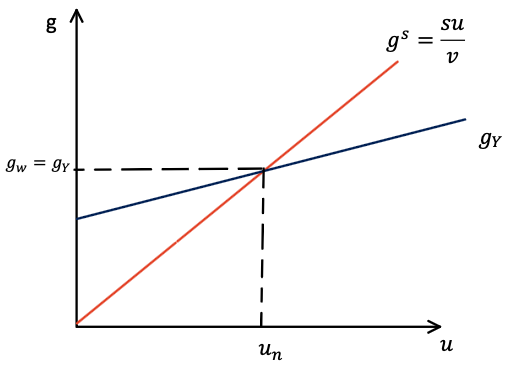
\includegraphics[width=0.75\linewidth,height=\textheight,keepaspectratio]{figuras/equilibrio_harrod.png}

}

\caption{\label{fig-equilibrio-harrod}Equilíbrio no modelo de Harrod:
interseção entre poupança e investimento.}

\end{figure}%

É importante notar que a condição para o equilíbrio acontecer é: \[ 
\begin{aligned}
g_y &= g_W\\
\frac{su}{v}&=\frac{s u_n}{v}
\end{aligned}
\] O que nos leva à condição de: \[
\begin{aligned}
u &= u_n\\
\frac{Y}{Y_K} &= \frac{Y_n}{Y_K}\\
Y &= Y_n
\end{aligned}\]

Ou seja, que o nível de demanda efetiva convirja para o nível esperado,
tal como discutido nas expectativas de curto-prazo.

\section{A taxa natural de crescimento}\label{sec-natural-harrod}

Além da taxa efetiva e da taxa desejada, Harrod introduziu uma terceira
taxa: a \emph{taxa natural de crescimento} (\(g_n\)). Esta taxa
representa o limite máximo de crescimento imposto pelo lado da oferta,
ou seja, pelas condições de disponibilidade de fatores de produção.

Imagine uma pequena aldeia. Sua capacidade produtiva dependerá
fundamentalmente de duas coisas:

\begin{enumerate}
\def\labelenumi{\arabic{enumi}.}
\tightlist
\item
  \textbf{Da quantidade de pessoas existentes}: mais trabalhadores
  disponíveis permitem produzir mais.
\item
  \textbf{Da tecnologia utilizada na produção}: melhores técnicas
  produtivas aumentam a produtividade do trabalho.
\end{enumerate}

Portanto, o crescimento da capacidade produtiva desta aldeia dependerá
do crescimento populacional e do desenvolvimento tecnológico.
Formalmente:

\begin{equation}\protect\phantomsection\label{eq-gn-harrod}{\boxed{g_n = g_L + g_A}}\end{equation}

onde:

\begin{itemize}
\tightlist
\item
  \(g_L\) é a taxa de crescimento da força de trabalho (população);
\item
  \(g_A\) é a taxa de progresso tecnológico (aumento da produtividade).
\end{itemize}

Harrod assumiu que a tecnologia é do tipo \emph{Harrod-neutra}, o que
significa que:

\begin{enumerate}
\def\labelenumi{\arabic{enumi}.}
\tightlist
\item
  a relação capital-produto (\(v\)) permanece constante;
\item
  a distribuição funcional da renda não é afetada pelo progresso
  técnico;
\item
  o produto cresce proporcionalmente ao crescimento tecnológico.
\end{enumerate}

\section{O primeiro problema de Harrod: a instabilidade da taxa
garantida}\label{sec-primeiro-problema-harrod}

O modelo de Harrod apresenta o que a literatura convencional chama de
``primeiro problema'': a instabilidade da taxa garantida de crescimento.

O problema pode ser enunciado da seguinte forma: o ponto de equilíbrio
definido pela igualdade \(g_Y = g_W\) é estável? A resposta de Harrod é
negativa. Sempre que a taxa efetiva de crescimento se desvia da taxa
garantida, forças centrífugas atuam para ampliar o desvio, e não para
corrigi-lo.

\subsection{O mecanismo da
instabilidade}\label{o-mecanismo-da-instabilidade}

Para entender a instabilidade, precisamos incorporar ao modelo o
\emph{princípio do acelerador}. Harrod propôs uma função de investimento
em que a taxa efetiva de crescimento depende da diferença entre o grau
de utilização efetivo e o grau de utilização normal:

\begin{equation}\protect\phantomsection\label{eq-acelerador-harrod}{g_Y = \gamma_0 + \gamma_u (u - u_n), \quad \gamma_0, \gamma_u > 0}\end{equation}

onde:

\begin{itemize}
\tightlist
\item
  \(\gamma_0\) é a taxa de crescimento autônoma (ou componente de
  expectativas representando o ``espírito animal'');
\item
  \(\gamma_u\) mede a sensibilidade do investimento a desvios do grau de
  utilização em relação ao desejado;
\item
  \((u - u_n)\) é o desvio do grau de utilização.
\end{itemize}

Além disso, Harrod assumiu que as expectativas se ajustam de acordo com
o desvio observado:

\begin{equation}\protect\phantomsection\label{eq-ajuste-expectativas}{\Delta \gamma_0 = v (u - u_n)}\end{equation}

A intuição por trás desse mecanismo é a seguinte:

\begin{enumerate}
\def\labelenumi{\arabic{enumi}.}
\tightlist
\item
  Se \(u > u_n\) (economia operando acima da capacidade planejada), as
  firmas observam que estão vendendo mais do que o planejado,
  verificando variações não desjeadas de seus estoques.
\item
  Isso melhora suas expectativas de demanda futura.
\item
  Elas decidem acelerar o investimento para expandir a capacidade
  produtiva.
\item
  O aumento do investimento aquece ainda mais a economia, elevando ainda
  mais o grau de utilização.
\item
  O processo se retroalimenta, afastando a economia cada vez mais do
  equilíbrio.
\end{enumerate}

O oposto também é verdadeiro: se \(u < u_n\), as firmas observam que
estão vendendo menos do que o planejado, pioram suas expectativas,
reduzem o investimento, a economia desacelera e o grau de utilização cai
ainda mais.

\begin{tcolorbox}[enhanced jigsaw, arc=.35mm, bottomrule=.15mm, bottomtitle=1mm, breakable, colback=white, colbacktitle=quarto-callout-warning-color!10!white, colframe=quarto-callout-warning-color-frame, coltitle=black, left=2mm, leftrule=.75mm, opacityback=0, opacitybacktitle=0.6, rightrule=.15mm, title=\textcolor{quarto-callout-warning-color}{\faExclamationTriangle}\hspace{0.5em}{Por que a instabilidade é um problema?}, titlerule=0mm, toprule=.15mm, toptitle=1mm]

A instabilidade é considerada um problema porque torna o modelo de
Harrod pouco útil para a análise empírica. Se o equilíbrio é instável, a
economia tenderá a se afastar dele sempre que ocorrer um desvio mínimo,
o que torna a trajetória de equilíbrio uma ``faca de dois gumes''
(\emph{knife-edge}).

Em outras palavras: se a economia não estiver exatamente sobre a
trajetória de crescimento garantido, ela tende a explodir para cima
(euforia) ou para baixo (frustração).

\end{tcolorbox}

\subsection{Representação gráfica da
instabilidade}\label{representauxe7uxe3o-gruxe1fica-da-instabilidade}

Graficamente, o primeiro problema de Harrod pode ser representado da
seguinte forma:

\begin{figure}

\centering{

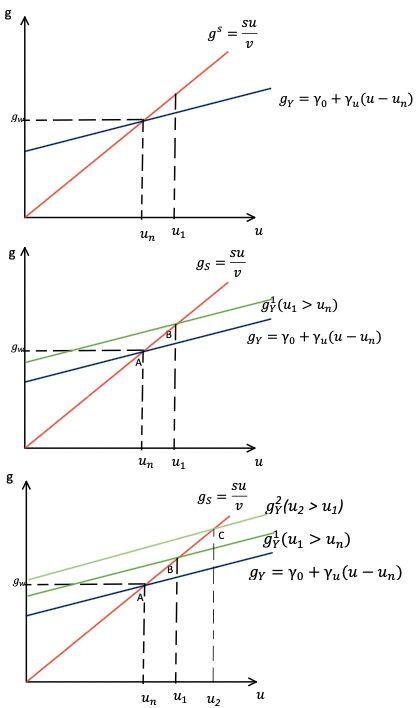
\includegraphics[width=1\linewidth,height=\textheight,keepaspectratio]{figuras/instabilidade_harrod.png}

}

\caption{\label{fig-instabilidade-harrod}Instabilidade do modelo de
Harrod.}

\end{figure}%

No ponto \(A\), a curva de poupança (\(g_S\)) e a curva de investimento
\((g_Y)\) se interceptam no grau normal de utilização (\(u_n\)). Este é
o equilíbrio.

No entanto, suponha que, por alguma razão, a curva de investimento se
desloque para \(g_Y^1\). O novo equilíbrio ocorre em \(B\), com um grau
de utilização \(u_1 > u_n\). As firmas observam que estão vendendo mais
do que o esperado, melhoram suas expectativas, e a curva de investimento
se desloca para \(g_Y^2\), gerando um novo equilíbrio com \(u_2 > u_1\).
O processo se repete, afastando cada vez mais a economia do equilíbrio
inicial.

Analogamente, se a curva de investimento se deslocasse para baixo, o
processo operaria em sentido contrário, com a economia se afastando para
baixo.

Em seu ensaio, Harrod resume este resultado da seguinte forma:

\begin{quote}
``The dynamic theory so far stated may be summed up in two propositions.
(i) A unique warranted line of growth is determined jointly by the
propensity to save and the quantity of capital required by technological
and other considerations per unit increment of total output. Only if
producers keep to this line will they find that on balance their
production in each period has been neither excessive nor deficient. (ii)
On either side of this line is a `field' in which centrifugal forces
operate, the magnitude of which varies directly as the distance of any
point in it from the warranted line. Departure from the warranted line
sets up an inducement to depart farther from it. The moving equilibrium
of advance is thus a highly unstable one.'' (Harrod 1939, p.~23)
\end{quote}

Representando a dinâmica por um diagrama de fases, temos a
Figura~\ref{fig-fases-harrod}.

\begin{figure}

\centering{

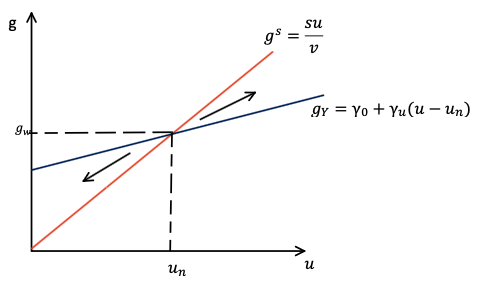
\includegraphics[width=0.75\linewidth,height=\textheight,keepaspectratio]{figuras/fases_harrod.png}

}

\caption{\label{fig-fases-harrod}Instabilidade do modelo de Harrod.}

\end{figure}%

Em que notamos que qualqeur ponto inicial em que a demanda efetiva não
seja compatível com as expectativas dos agentes conduz a economia para
um processo explosivo. Portanto, é possível transpor a teoria estática
de Keynes para uma teoria dinâmica e estável? sim, mas só se você
assumir que o equilíbrio do curto prazo esteja ocorrendo. Pois, qualquer
ponto de partida distinto desse conduziria a economia para um estado de
euforia ou para uma dperessão profunda.

\section{O segundo problema de Harrod: a divergência entre a taxa
garantida e a taxa natural}\label{sec-segundo-problema-harrod}

Mesmo que a economia consiga, por algum acaso, se manter sobre a
trajetória de crescimento garantido, ainda assim o equilíbrio pode não
ser sustentável. Este é o chamado ``segundo problema'' de Harrod: a
possível divergência entre a taxa garantida (\(g_W\)) e a taxa natural
(\(g_n\)).

\[g_y= g_W \neq g_n\]

\subsection{Caso 1: A taxa natural supera a taxa
garantida}\label{caso-1-a-taxa-natural-supera-a-taxa-garantida}

\begin{figure}

\centering{

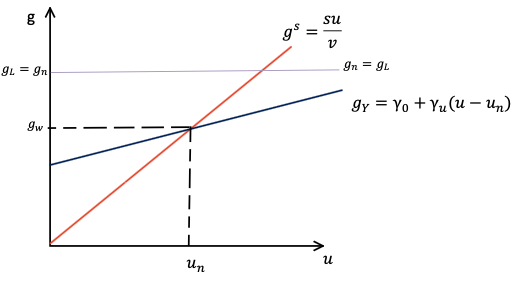
\includegraphics[width=1\linewidth,height=\textheight,keepaspectratio]{figuras/harrod_caso1.png}

}

\caption{\label{fig-harrod-caso1}Taxa garantida abaixo da taxa natural.}

\end{figure}%

Se \(g_n > g_W\), a economia cresce a uma taxa inferior ao seu potencial
máximo. Por simplicidade, podemos assumir que \(g_A=0\) e que o
crescimento natural é dado apenas pelo crescimento populacional.

Este caso implica que a taxa de crescimento populacional é mais rápida
do que a taxa de expansão da demanda efetiva. Significa que a taxa de
pessoas entrando na força de trabalho está maior do que a taxa que faz
com que as firmas contratem novas pessoas.

Neste caso, a economia tenderá a operar com desemprego crescente ao
longo do tempo. Mesmo que, por acaso, a taxa efetiva se iguale à
garantida, a economia não será capaz de absorver toda a força de
trabalho disponível.

\subsection{Caso 2: A taxa natural é inferior à taxa
garantida}\label{caso-2-a-taxa-natural-uxe9-inferior-uxe0-taxa-garantida}

\begin{figure}

\centering{

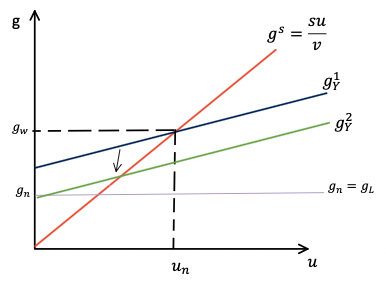
\includegraphics[width=1\linewidth,height=\textheight,keepaspectratio]{figuras/harrod_caso2.png}

}

\caption{\label{fig-harrod-caso2}Taxa garantida acima da taxa natural.}

\end{figure}%

Se \(g_n < g_W\), a economia cresce a uma taxa superior ao seu potencial
máximo. A demanda efetiva se expande mais rapidamente do que a
capacidade produtiva.

Pense que a taxa em que as empresas contratam novas pessoas superará a
taxa de pessoas entrando na força de trabalho. Esta situação pode até
permanecer enquanto houver um estoque de desempregados, mas tão logo
este estoque se esgote, mesmo que haja demanda pelo produto, não terá
mão-de-obra disponível para produzí-lo.

Neste caso, a taxa de estado estacionário encontrará um limite na
mão-de-obra disponível em algum momento. Quando isso acontecer, a
demanda cairá, reduzindo o grau de utilização da capacidade.

O problema aqui é duplo:

\begin{enumerate}
\def\labelenumi{\arabic{enumi}.}
\tightlist
\item
  A economia eventualmente esbarra no limite imposto pela oferta de
  trabalho.
\item
  Quando isso ocorre, o grau de utilização cai abaixo do normal, o que
  ativa o mecanismo do primeiro problema de Harrod: a instabilidade.
\end{enumerate}

Ou seja, o segundo problema não é independente do primeiro. Uma vez que
a taxa garantida supera a natural, a economia está fadada a colidir com
o limite da oferta, gerando uma crise que a joga para baixo da
trajetória de equilíbrio.

\section{A dupla condição de equilíbrio}\label{sec-dupla-condicao}

Para que o modelo de Harrod apresente um equilíbrio dinâmico estável,
duas condições precisariam ser satisfeitas simultaneamente:

\begin{enumerate}
\def\labelenumi{\arabic{enumi}.}
\tightlist
\item
  \(g_Y = g_W\) (a taxa efetiva deve igualar a desejada)
\item
  \(g_W = g_n\) (a taxa desejada deve igualar a natural)
\end{enumerate}

Ou, de forma combinada:

\begin{equation}\protect\phantomsection\label{eq-dupla-condicao}{g_L + g_A = g_W = g_Y = \frac{s u}{v} = \frac{s u_n}{v}}\end{equation}

O que garante que essas duas condições sejam satisfeitas? A resposta de
Harrod é: \emph{nada}. Não há mecanismo automático que assegure a
coincidência entre a taxa desejada e a natural.

\begin{tcolorbox}[enhanced jigsaw, arc=.35mm, bottomrule=.15mm, bottomtitle=1mm, breakable, colback=white, colbacktitle=quarto-callout-important-color!10!white, colframe=quarto-callout-important-color-frame, coltitle=black, left=2mm, leftrule=.75mm, opacityback=0, opacitybacktitle=0.6, rightrule=.15mm, title=\textcolor{quarto-callout-important-color}{\faExclamation}\hspace{0.5em}{A ``faca de dois gumes'' de Harrod}, titlerule=0mm, toprule=.15mm, toptitle=1mm]

A necessidade de que duas condições exógenas e independentes coincidam é
o que torna o modelo de Harrod uma ``faca de dois gumes''
(\emph{knife-edge}). A economia só cresce de forma equilibrada se:

\begin{enumerate}
\def\labelenumi{\arabic{enumi}.}
\tightlist
\item
  as decisões descentralizadas de investimento gerarem exatamente a taxa
  de crescimento desejada;
\item
  a taxa desejada coincidir com a taxa natural.
\end{enumerate}

A probabilidade de que ambas as condições sejam atendidas
simultaneamente é extremamente baixa.

\end{tcolorbox}

\section{Avaliação do modelo de Harrod}\label{sec-avaliacao-harrod}

O modelo de Harrod foi objeto de inúmeras críticas e interpretações. A
avaliação mais amplamente aceita é que Harrod não apresentou uma teoria
completa de crescimento e distribuição, mas sim um arcabouço
metodológico fundamental.

\subsection{As limitações do
modelo}\label{as-limitauxe7uxf5es-do-modelo}

Autores como Kregel (1971), Asimakopulos (1991) e Besomi (2001)
apontaram as seguintes limitações:

\begin{enumerate}
\def\labelenumi{\arabic{enumi}.}
\tightlist
\item
  \textbf{Ausência de uma teoria da distribuição}: a distribuição
  funcional da renda é tratada como dada, não explicada pelo modelo.
\item
  \textbf{Determinação insuficiente do investimento}: o princípio do
  acelerador, embora importante, não é suficiente para explicar as
  decisões de investimento.
\item
  \textbf{Falta de consideração da taxa de juros e dos custos de
  financiamento}: o modelo ignora o papel do sistema financeiro.
\item
  \textbf{Falta de consideração da taxa de lucro}: o modelo não
  incorpora a lucratividade como determinante do investimento.
\item
  \textbf{Tratamento da relação capital-produto como constante}: Harrod
  assume que \(v\) é fixo, o que exclui a possibilidade de mudanças
  técnicas que alterem essa relação.
\end{enumerate}

\subsection{A contribuição de
Harrod}\label{a-contribuiuxe7uxe3o-de-harrod}

Apesar dessas limitações, a contribuição de Harrod foi fundamental para
o desenvolvimento da teoria econômica pós-keynesiana:

\begin{enumerate}
\def\labelenumi{\arabic{enumi}.}
\tightlist
\item
  \textbf{Estabeleceu a distinção entre três taxas de crescimento}:
  efetiva, garantida e natural.
\item
  \textbf{Mostrou que o equilíbrio dinâmico keynesiano não é
  automaticamente estável}.
\item
  \textbf{Identificou a necessidade de mecanismos de ajuste adicionais}
  (distribuição, expectativas) para estabilizar o sistema.
\item
  \textbf{Forneceu um arcabouço metodológico para o estudo da dinâmica
  econômica}.
\end{enumerate}

Como bem resumiu Kregel:

\begin{quote}
``Harrod has provided a much needed methodological approach and a
valuable start towards placing the General Theory in a dynamic context.
The idea that the warranted and the natural rate are not necessarily the
same or equal and the complications that arise when they are not ranks
as a basic contribution to growth.'' (Kregel 1971, p.~118)
\end{quote}

Além do que, o obejtivo de Harrod era estabelecer as condições de
equilíbrio do modelo para entender os fatores que o desestabilizariam. A
ideia final, que Harrod não chegou a desenvolver, era fazer sugestões de
política econômica. Ora, se o autor conseguisse mapear os elementos que
tornam o sistema instável, poderia então propor políticas para
neutralizar tais elementos e tornar a economia capitalista mais estável.

Este último obejtivo nunca cehgou a ser alcançado por Harrod, mas foi
desenvolvido por outros autores, como veremos ao longo desta apostila.

Por fim, para quem pensa que o objetivo e Harrod era montar um modelo de
crescimento para explicar ume stado estacinário de longo prazo, de fato
o modelo carrega sérios problemas. Contudo, se o objetivo do modelo de
Harrod fosse de fato explicar como a economia capitalista é
inerentemente instável, a sua contribuição foi mostrar que a
estabildiade da economia depende de uma variável tão fugaz quanto as
expectativas empresariais.

\section{Conexão com os modelos subsequentes}\label{sec-conexao-harrod}

O modelo de Harrod estabeleceu as bases para o desenvolvimento de outras
tradições teóricas:

\subsection{O modelo neoclássico de
Solow}\label{o-modelo-neocluxe1ssico-de-solow}

Solow (1956) interpretou o problema de Harrod como resultado da hipótese
de proporções fixas na produção (\(v\) constante). Ao permitir a
substituição entre capital e trabalho, Solow mostrou que a economia
poderia convergir para um estado estacionário com pleno emprego,
independentemente da taxa garantida.

Essa interpretação, no entanto, foi criticada por autores
pós-keynesianos por assumir que a substituição entre fatores ocorreria
de forma automática, sem considerar a incerteza fundamental e a rigidez
dos preços relativos.

\subsection{O modelo Kaleckiano de
crescimento}\label{o-modelo-kaleckiano-de-crescimento}

O modelo Kaleckiano (discutido no Capítulo~\ref{sec-modelo-kal}) partiu
da mesma crítica de Harrod em relação à instabilidade, mas propôs uma
solução diferente: a endogeneidade do grau de utilização de equilíbrio.

No modelo Kaleckiano, a taxa de crescimento não é determinada por uma
``faca de dois gumes'', mas pela interação entre a demanda efetiva e a
distribuição funcional da renda. Este modelo será aprofundado no
Capítulo~\ref{sec-modelo-kal}.

\subsection{O modelo Kaldor-Robinson}\label{o-modelo-kaldor-robinson}

O modelo Kaldor-Robinson, por sua vez, adotou a solução de ajuste pela
distribuição funcional da renda, desenvolvendo uma teoria em que a
participação dos lucros na renda se ajusta para garantir a igualdade
entre poupança e investimento na taxa natural.

\bookmarksetup{startatroot}

\chapter{Modelo Kaleckiano Canônico}\label{sec-modelo-kal}

\section{A Determinação dos Lucros e da Renda Nacional em
Kalecki}\label{sec-renda}

Esta seção apresenta, de forma didática, a teoria kaleckiana da
determinação dos lucros e da renda nacional, baseada em Hein (2014).

Kalecki distingue duas questões fundamentais: (i) o nível dos lucros,
determinado pela demanda efetiva, especialmente pelo investimento;(ii) a
distribuição funcional da renda, determinada pelo grau de monopólio
(\emph{markup}). Assim, é possível alterar a participação dos lucros na
renda sem alterar, necessariamente, o montante absoluto de lucros.

Partindo da identidade da renda,

\[\Pi + W = C_w + C_{\pi} + I\]

reorganizando os termos,

\[\Pi = C_w - W + C_{\pi} + I\]

Como a poupança dos trabalhadores é definida por \(S_w = W - C_w,\)
segue que

\[\Pi = C_{\pi} + I - S_w.\]

Assumindo que os trabalhadores gastam integralmente sua
renda,\(S_w = 0,\) obtém-se:

\begin{equation}\protect\phantomsection\label{eq-lucros}{\Pi = C_{\pi} + I.}\end{equation}

\begin{tcolorbox}[enhanced jigsaw, arc=.35mm, bottomrule=.15mm, bottomtitle=1mm, breakable, colback=white, colbacktitle=quarto-callout-note-color!10!white, colframe=quarto-callout-note-color-frame, coltitle=black, left=2mm, leftrule=.75mm, opacityback=0, opacitybacktitle=0.6, rightrule=.15mm, title=\textcolor{quarto-callout-note-color}{\faInfo}\hspace{0.5em}{Princípio da demanda efetiva}, titlerule=0mm, toprule=.15mm, toptitle=1mm]

Nesta expressão aparece uma das ideias centrais da teoria kaleckiana: os
capitalistas podem decidir quanto gastar, mas não podem decidir quanto
lucrar no período subsequente. O gasto autônomo antecede a renda e
determina o montante de lucros realizado pela economia.

\end{tcolorbox}

A Equação~\ref{eq-lucros} expressa o princípio da demanda efetiva,
contrariando diretamente a Lei de Say. A partir dela, Kalecki conclui
que os capitalistas podem decidir gastar mais no período subsequente,
mas não podem decidir obter maiores lucros. A única variável
verdadeiramente autônoma é o gasto; a renda e os lucros são determinados
posteriormente pelo processo multiplicador.

Daí decorre o conhecido aforismo atribuído a Kaldor:

\begin{quote}
\emph{Os capitalistas ganham o que gastam e os trabalhadores gastam o
que ganham.}
\end{quote}

É importante notar a generalidade do princípio da demanda efetiva. Não
se trata apenas da ideia de que o gasto dos capitalistas gera lucros. Em
termos mais amplos, a renda macroeconômica é determinada pelos gastos
que a antecedem.Macroeconomicamente, portanto, é incorreto afirmar que
um gasto decorre de uma renda previamente existente. A renda somente
passa a existir quando algum agente realiza um gasto. Caso esse gasto
não ocorra, a renda correspondente também não existirá. O gasto decorre
de um poder de compra concedido por algum agente hierarquicamente
superior e, uma vez realizado, gera uma renda de igual valor. Essa
renda, por sua vez, origina uma poupança exatamente igual ao gasto
inicial.

\begin{tcolorbox}[enhanced jigsaw, arc=.35mm, bottomrule=.15mm, bottomtitle=1mm, breakable, colback=white, colbacktitle=quarto-callout-important-color!10!white, colframe=quarto-callout-important-color-frame, coltitle=black, left=2mm, leftrule=.75mm, opacityback=0, opacitybacktitle=0.6, rightrule=.15mm, title=\textcolor{quarto-callout-important-color}{\faExclamation}\hspace{0.5em}{Generalização}, titlerule=0mm, toprule=.15mm, toptitle=1mm]

O princípio da demanda efetiva pode ser generalizado dizendo que as
variáveis de demanda determinam as variáveis de oferta.

Assim,

\begin{itemize}
\tightlist
\item
  o gasto gera a renda;
\item
  o investimento gera a poupança;
\item
  o gasto dos capitalistas gera os lucros;
\item
  o gasto público gera a arrecadação tributária;
\item
  e assim sucessivamente.
\end{itemize}

\end{tcolorbox}

Suponha agora que o consumo dos capitalistas seja uma fração constante
de seus lucros,

\[C_{\pi} = c_{\pi} \Pi.\]

Substituindo essa expressão na equação dos lucros,

\[\Pi = c_{\pi}\Pi + I.\]

Isolando os lucros,

\[\Pi = \frac{I}{1-c_{\pi}}.\]

Como a propensão a poupar dos capitalistas é definida por

\[s_c = 1-c_{\pi},\]

segue que

\begin{equation}\protect\phantomsection\label{eq-multlucros}{\Pi = \frac{I}{s_c}.}\end{equation}

Esta expressão corresponde ao \textbf{primeiro multiplicador
kaleckiano}. Quanto menor for a propensão a poupar dos capitalistas,
maior será o volume de lucros gerado para um mesmo nível de investimento
(os capitalistas ganham o que gastam).

Dividindo os lucros pela renda, obtém-se uma aproximação da participação
dos lucros na renda (\emph{profit-share}), o que pode ser expressa como
\(\pi=\frac{\Pi}{Y}\). Substituindo essa definição na expressão
anterior,

\[\begin{aligned}
\pi=\frac{I}{Ys_\pi} \\
\pi Y s_\pi = I\\
Y=\frac{I}{s_\pi \pi}
\end{aligned}\]

Também é possível obter esse resultado partindo da identidade
macroeconômica

\[I=S,\]

e assumindo que toda a poupança provém dos lucros,

\[I=s_\pi\Pi=s_\pi\pi Y\]

Logo,

\begin{equation}\protect\phantomsection\label{eq-multrenda}{Y=\frac{I}{s_\pi\pi}.}\end{equation}

Esta expressão representa o \textbf{multiplicador da renda kaleckiano},
mostrando como o investimento determina o nível de renda de equilíbrio.

O paradoxo da parcimônia (\emph{Paradox of Thrift}) permanece válido.
Caso os capitalistas aumentem sua propensão a poupar, o multiplicador
diminui, reduzindo a renda e os próprios lucros.

Kalecki também argumentou que, quando o investimento é financiado por
crédito bancário, o próprio processo de gasto gera os depósitos
necessários para liquidar posteriormente esse crédito. Dessa forma, o
investimento cria a poupança correspondente (\emph{investment finances
itself}), antecipando ideias posteriormente desenvolvidas pela teoria
pós-keynesiana do circuito monetário.

Por fim, considere um aumento do grau de oligopólio, elevando o
\emph{markup}. Pela teoria de preços de Kalecki, isso aumenta o
\emph{profit-share} \((\pi)\). Entretanto, mantendo constante o
investimento autônomo, o primeiro multiplicador (ver
Equação~\ref{eq-multlucros}) mostra que o montante de lucros permanece
inalterado. O ajuste ocorre por meio do multiplicador da renda
(Equação~\ref{eq-multrenda}), de modo que um aumento da participação dos
lucros reduz o nível de renda de equilíbrio, embora o montante absoluto
de lucros permaneça constante \(\pi\uparrow=\frac{\Pi}{Y\downarrow}\).

\begin{tcolorbox}[enhanced jigsaw, arc=.35mm, bottomrule=.15mm, bottomtitle=1mm, breakable, colback=white, colbacktitle=quarto-callout-note-color!10!white, colframe=quarto-callout-note-color-frame, coltitle=black, left=2mm, leftrule=.75mm, opacityback=0, opacitybacktitle=0.6, rightrule=.15mm, title=\textcolor{quarto-callout-note-color}{\faInfo}\hspace{0.5em}{Resultado fundamental}, titlerule=0mm, toprule=.15mm, toptitle=1mm]

Uma das contribuições centrais de Kalecki consiste em distinguir
claramente:

\begin{itemize}
\tightlist
\item
  o \textbf{nível dos lucros}, determinado pela demanda efetiva; e
\item
  a \textbf{participação dos lucros na renda}, determinada pelo grau de
  monopólio (\emph{markup}).
\end{itemize}

Esses dois conceitos não devem ser confundidos.

\end{tcolorbox}

\section{A Formação de preços e distribuição de
renda}\label{sec-formacao-precos}

Se a renda é determinada pela distribuição e pelos gastos, então não
será o nível de renda que determinará os preços, como pressupõem as
teorias de inflação de demanda. Precisamos, portanto, compreender como
ocorre a formação dos preços e como ela determina a distribuição
funcional da renda.

A teoria neoclássica parte da hipótese de concorrência perfeita para
justificar uma curva de custos médios em formato de ``U''. À medida que
a produção aumenta, chega-se a um ponto em que a escassez dos fatores
produtivos provoca elevação dos custos variáveis e, consequentemente, do
custo médio.
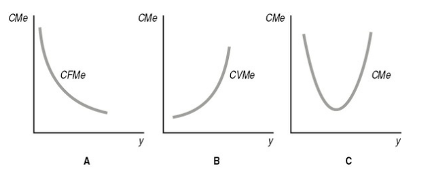
\includegraphics[width=0.8\linewidth,height=\textheight,keepaspectratio,alt={Curva de custos neoclássica}]{figuras/custosneo.png}

A teoria kaleckiana rejeita essa hipótese. Em vez de assumir mercados
perfeitamente competitivos, Kalecki parte da ideia de que o capitalismo
é inerentemente concentrado e que as firmas possuem poder de mercado.

Dessa forma, a curva de custos da firma pode ser representada por dois
trechos distintos:

\begin{itemize}
\tightlist
\item
  um trecho aproximadamente horizontal, no qual a existência de
  capacidade ociosa permite ampliar a produção sem aumentos
  significativos dos custos;
\item
  um trecho ascendente, quando a produção se aproxima da plena
  capacidade.
\end{itemize}

\begin{figure}

\centering{

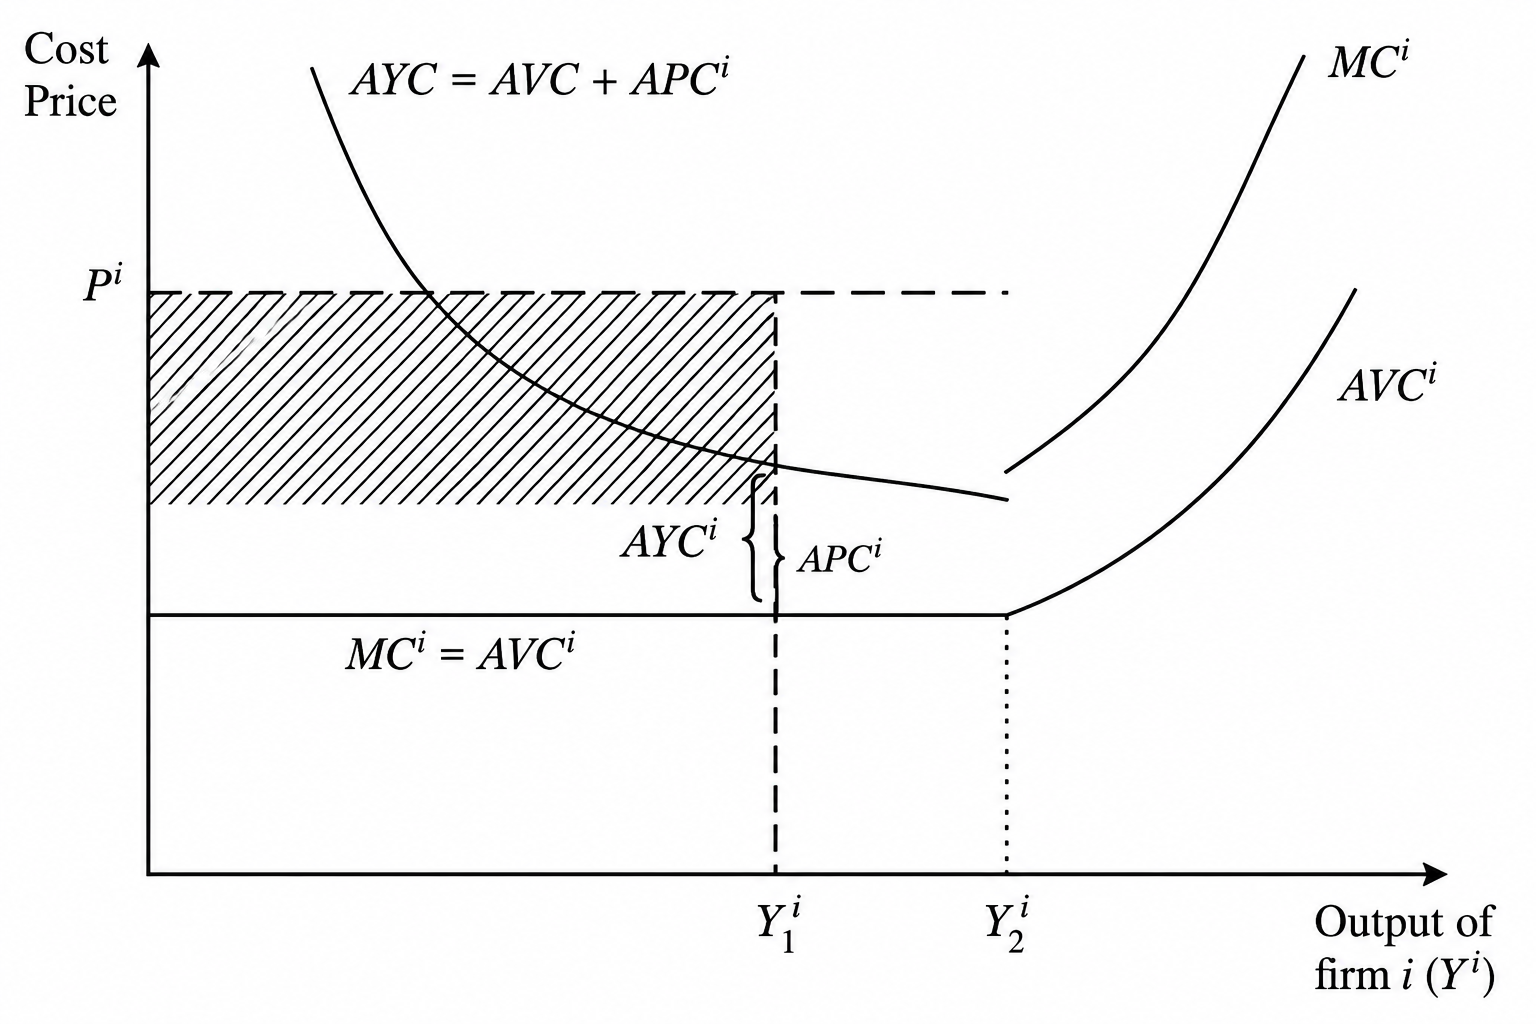
\includegraphics[width=0.8\linewidth,height=\textheight,keepaspectratio]{figuras/custoskale.png}

}

\caption{\label{fig-custoskale}Curva de custos kaleckiana}

\end{figure}%

Como consequência, as empresas normalmente optam por operar abaixo da
plena utilização da capacidade produtiva, preservando uma margem de
segurança para responder a aumentos inesperados da demanda sem perder
participação de mercado.

\begin{tcolorbox}[enhanced jigsaw, arc=.35mm, bottomrule=.15mm, bottomtitle=1mm, breakable, colback=white, colbacktitle=quarto-callout-note-color!10!white, colframe=quarto-callout-note-color-frame, coltitle=black, left=2mm, leftrule=.75mm, opacityback=0, opacitybacktitle=0.6, rightrule=.15mm, title=\textcolor{quarto-callout-note-color}{\faInfo}\hspace{0.5em}{Capacidade ociosa planejada}, titlerule=0mm, toprule=.15mm, toptitle=1mm]

A existência de capacidade ociosa não é interpretada como uma
imperfeição temporária do mercado, mas como uma característica normal do
funcionamento das economias capitalistas. Ela constitui um elemento
central da teoria kaleckiana da firma.

\end{tcolorbox}

O ponto de pleno emprego, no entanto, não é intransponível, mas costuma
ser evitado pelos altos custos envolvidos. A partir do ponto de pleno
emprego, os insumos ficam mais difíceis de serem acessados, as máquinas
começam a quebrar com mais facilidade, os custos trabalhistas sobem e
vários ônus são gerados. Como em tempos de guerra, as firmas até
conseguem operar acima da plena capacidade, mas evitam.

Nessas condições, os preços deixam de ser determinados pelo equilíbrio
entre oferta e demanda e passam a ser definidos pela aplicação de uma
margem de \emph{mark-up} sobre os custos unitários de produção. Estes
custos unitários envolvem tanto os salários por unidade produzida
\((w \frac{L}{Y} = wa)\) como os custos intermediários \((\mu)\), que
podem ser interpretados como matérias-primas quando analisamos uma firma
individual ou como insumos importados quando pensamos em uma economia
aberta.

Escrevemos, então,

\begin{equation}\protect\phantomsection\label{eq-precos}{P=(1+ \tau)(wa+ p_\mu \mu)}\end{equation}

em que

\begin{itemize}
\tightlist
\item
  \(P\) representa o preço do produto;
\item
  \(w\) é a taxa de salário nominal;
\item
  \(a\) corresponde ao requisito unitário de trabalho;
\item
  \(wa\) representa o custo unitário do trabalho;
\item
  \(m\) representa os custos intermediários por unidade produzida;
\item
  \(j\) é a margem de \emph{mark-up}.
\end{itemize}

Para estudar a relação entre a teoria de preços de Kalecki e a
distribuição de renda podemos manipular a equação acima multiplicando-a
por \(\frac{wa}{wa}\). Mas antes precisamos simplificar a relação de
custo da matéria-prima por custo unitário como: \[j=\frac{p_\mu}{wa}\]

Substituindo essa definição na Equação Equação~\ref{eq-precos}, obtemos

\[\begin{aligned}
p = (1+\tau) \left({wa}+p_\mu \mu \frac{wa}{wa}\right)\\
p = (1+\tau) \left({wa}\left(1+\frac{p_\mu\mu}{wa}\right)\right)\\
p=(1+\tau)(wa(1+j))
\end{aligned}\]

A margem de lucro por unidade produzida pode então ser escrita como

\[\begin{aligned}
\frac{\Pi}{Y}=\tau(wa(1+j))\\
\frac{\Pi}{Y}=\tau wa(1+j)
\end{aligned}\]

Entretanto, ainda não podemos interpretar essa expressão como a
participação dos lucros na renda (\emph{profit share}), pois ela
considera o valor bruto da produção, e não o valor adicionado.

O \emph{profit share} é definido como

\[\pi=\frac{\Pi}{\Pi+W}.\] Dividindo todo mundo por \(Y\):
\[\pi=\frac{\frac{\Pi}{Y}}{\frac{\Pi}{Y}+\frac{wL}{Y}}.\]

Substituindo as expressões para lucros e salários por unidade produzida,
chega-se ao resultado

\begin{equation}\protect\phantomsection\label{eq-profit-share}{\begin{aligned}
\pi=\frac{\tau wa (1+j)}{\tau wa(1+j)+wa}\\
\pi=\frac{\tau(1+j)}{\tau(1+j)+1}\\
\pi = \frac{\tau}{\frac{1}{1+j} + \tau}
\end{aligned}}\end{equation}

De forma equivalente, a participação dos salários na renda (\emph{wage
share}) é dada por

\[\begin{aligned}
1-\pi=\frac{W}{\Pi+W}\\
1-\pi = \frac{wa}{\tau wa(1+j) + wa}\\
1-\pi = \frac{1}{\tau(1+j)+1}
\end{aligned}\]

Esses resultados mostram que a distribuição funcional da renda depende
fundamentalmente de dois fatores:

\begin{enumerate}
\def\labelenumi{\arabic{enumi}.}
\tightlist
\item
  do grau de \emph{mark-up} praticado pelas firmas \((\tau)\);
\item
  da importância relativa dos custos intermediários na produção \((j)\).
\end{enumerate}

\begin{tcolorbox}[enhanced jigsaw, arc=.35mm, bottomrule=.15mm, bottomtitle=1mm, breakable, colback=white, colbacktitle=quarto-callout-important-color!10!white, colframe=quarto-callout-important-color-frame, coltitle=black, left=2mm, leftrule=.75mm, opacityback=0, opacitybacktitle=0.6, rightrule=.15mm, title=\textcolor{quarto-callout-important-color}{\faExclamation}\hspace{0.5em}{Resultado fundamental}, titlerule=0mm, toprule=.15mm, toptitle=1mm]

Na teoria kaleckiana, a distribuição funcional da renda não decorre da
produtividade marginal dos fatores de produção.

Ela é determinada pelo processo de formação de preços adotado pelas
firmas.

Em outras palavras, a inflação de custos define a distribuição funcional
da renda.

\end{tcolorbox}

Em uma economia fechada, na qual desconsideramos custos intermediários
importados \((j=0)\), podemos reduzir a Equação~\ref{eq-profit-share} à:

\begin{equation}\protect\phantomsection\label{eq-pi}{\pi=\frac{\tau}{1+\tau}.}\end{equation}

Essa expressão evidencia que o aumento do \emph{mark-up} eleva
diretamente a participação dos lucros na renda.

O nível do \emph{mark-up} depende de diversos fatores institucionais e
estruturais da economia, entre os quais destacam-se:

\begin{itemize}
\tightlist
\item
  o grau de concentração industrial;
\item
  o grau de verticalização da produção;
\item
  a importância de formas de competição não relacionadas ao preço, como
  publicidade e diferenciação de produtos;
\item
  os \emph{overhead costs} das empresas;
\item
  o poder de barganha dos sindicatos.
\end{itemize}

Esses fatores serão tratados como exógenos ao longo do desenvolvimento
do modelo kaleckiano de crescimento, de modo que a distribuição
funcional da renda será considerada previamente determinada pelo
processo de formação de preços.

\bookmarksetup{startatroot}

\chapter{Modelo Neo-Kaleckiano (Bhaduri e Marglin)}\label{sec-modelo-bm}

\section{Introdução}\label{sec-introducao-bm}

O modelo neokaleckiano desenvolvido por Bhaduri e Marglin representa uma
das principais extensões da tradição kaleckiana de crescimento e
distribuição. Seu objetivo é incorporar, de forma explícita, o efeito da
distribuição funcional da renda sobre as decisões de investimento,
permitindo analisar diferentes regimes de demanda e crescimento.

O modelo parte da estrutura do modelo kaleckiano canônico, mas modifica
a função de investimento ao introduzir a participação dos lucros na
renda (\emph{profit share}) como um determinante autônomo do
investimento desejado. Essa modificação torna possível distinguir
economias em que aumentos da parcela dos lucros estimulam a atividade
econômica daquelas em que o crescimento é favorecido pelo aumento da
participação dos salários.

Ao final deste capítulo veremos que essa alteração aparentemente simples
produz resultados bastante ricos, permitindo diferenciar:

\begin{itemize}
\tightlist
\item
  regimes de demanda \emph{wage-led} e \emph{profit-led};
\item
  regimes de crescimento \emph{wage-led} e \emph{profit-led};
\item
  situações em que demanda e crescimento respondem de maneira distinta
  às mudanças distributivas.
\end{itemize}

\section{A crítica ao modelo kaleckiano canônico}\label{sec-critica-bm}

Este modelo parte da estrutura do modelo canônico, mas estabelce uma
divergênica importante a partir de uma crítica à função de investimento.
Bhaduri e Marglin apontaram que o modelo canônico de crescimento
kaleckiano superestima o papel da demanda efetiva e subestima o papel da
distribuição de renda sobre o investimento.

No modelo kaleckiano apresentado no capítulo anterior, o investimento
depende positivamente do grau de utilização da capacidade produtiva.
Para fins de praticidade, representaremos função de investimento
conforme o capítulo anterior do modelo canônico:

\[g_{K}=\gamma_0+\gamma_r r + \gamma_u u\]

em que:

\begin{itemize}
\tightlist
\item
  \(\gamma_0\) representa o componente autônomo do investimento;
\item
  \(\gamma_u>0\) mede a sensibilidade do investimento ao grau de
  utilização da capacidade;
\item
  \(u\) representa o grau de utilização.
\end{itemize}

Se lemrbarmos que \(r=\frac{\pi u}{v}\), podemos reescrever a equação
acima como:

\begin{equation}\protect\phantomsection\label{eq-gkcanonico}{\begin{aligned}
g_K=\gamma_0 + \gamma_r \frac{\pi u}{v} + \gamma_u u \\
g_K = \gamma_0 + \left(\gamma_r \frac{\pi}{v}+\gamma_u \right) u
\end{aligned}}\end{equation}

em que \(\pi\) representa a participação dos lucros na renda e \(v\)
corresponde à relação capital-produto.

Uma crítica inicial é que, conforme podemos constatar na
Equação~\ref{eq-gkcanonico}, o grau de utilização da capacidade tem
impacto duplo sobre o investimento. Quando a demanda efetiva aquece
\((u\uparrow)\), as firmas aumentam o investimento tanto pelo efeito
acelerador como pelo efeito lucratividade (ver termo entre parênteses na
Equação~\ref{eq-gkbm}).

Essa especificação sugere que o impacto será sempre amplificado, pois
pressupõe que sempre temos \(\gamma_u > 0\). Entretanto, essa relação
positiva entre grau de utilização e investimento possui uma relação
implícita nada trivial. O fato de \(\gamma_u\) se sempre positivo pode
ser interpretado como: \emph{tudo o mais constante} (\textbf{inclusive a
taxa de lucro}), o aumento do grau de utilização conduz ao aumento da
taxa de investimento.

Repare que manter a taxa de lucro constante após ocorrer o aumento do
grau de utilização só será possível se houver um aumento proporcional da
participação dos lucros na renda. Isso é mais fácil de ser verificado
pela representação algébrica:

\[\bar{r} = \frac{\pi \downarrow u\uparrow}{v}\]

No entanto, devemos lembrar que a parcela dos lucros na renda é
diretamente relacionada com a taxa de \emph{markup} (ver
Equação~\ref{eq-pi}). Ou seja, a relação descrita acima sugere que o
modelo kaleckiano admite, implicitamente, que uma firma pode observar
uma redução do seu \emph{markup} e, ainda assim, decidir ampliar seus
investimentos devido ao grau de utilização permanecer elevado.

Bhaduri e Marglin questionam precisamente essa hipótese.

\begin{tcolorbox}[enhanced jigsaw, arc=.35mm, bottomrule=.15mm, bottomtitle=1mm, breakable, colback=white, colbacktitle=quarto-callout-important-color!10!white, colframe=quarto-callout-important-color-frame, coltitle=black, left=2mm, leftrule=.75mm, opacityback=0, opacitybacktitle=0.6, rightrule=.15mm, title=\textcolor{quarto-callout-important-color}{\faExclamation}\hspace{0.5em}{A crítica de Bhaduri e Marglin}, titlerule=0mm, toprule=.15mm, toptitle=1mm]

Os autores argumentam que as firmas não observam apenas o grau de
utilização da capacidade ao decidir investir.

A distribuição funcional da renda (refletida na participação dos lucros
ou, equivalentemente, no \emph{markup}) também influencia as
expectativas de rentabilidade futura.

\end{tcolorbox}

\section{A função de investimento de Bhaduri e
Marglin}\label{sec-investimento-bm}

Como alternativa, Bhaduri e Marglin retomam a tradição inaugurada por
Joan Robinson. Segundo essa abordagem, o investimento depende da
\textbf{taxa de lucro esperada}, e não apenas da taxa de lucro
realizada.

Assumindo uma relação capital-produto constante, a taxa de lucro
esperada depende positivamente de:

\begin{itemize}
\tightlist
\item
  o grau de utilização da capacidade produtiva: \(u\);
\item
  a participação dos lucros na renda: \(\pi\).
\end{itemize}

Uma representação linear dessa hipótese pode ser escrita como:

\begin{equation}\protect\phantomsection\label{eq-gkbm}{g_K= \gamma_0 + \gamma_{\pi}\pi + \gamma_u u}\end{equation}

em que

\begin{itemize}
\tightlist
\item
  \(\gamma_{\pi}>0\); mede a sensibilidade do investimento à
  distribuição funcional da renda;
\item
  \(\gamma_u>0\); representa a resposta ao grau de utilização.
\end{itemize}

Nesta versão, a decisão de investimento depende não da taxa de lucro
realizada, mas da distribuição de renda desejada. Mesmo o \(\gamma_u\)
sendo positivo, como antes, ele já não mais pressupõe a manutenção da
taxa de lucro, pois o que influencia o investimento é a parcela dos
lucros, não sua taxa. Desta forma, pode ocorrer de a taxa de lucro
realizada ficar abaixo da que seria compatível com o markup desejado
pelas firmas, fato que desestimularia novos investimentos e reduziria a
taxa de crescimento do estoque de capital por meio do parâmtero
\(\gamma_\pi\).

Quando \(\gamma_{\pi}=0\), a Equação~\ref{eq-gkbm} reduz-se
aproximadamente à função de investimento estudada no capítulo anterior.
Aqui, basicamente, temos duas forças oeprando sobre o investimento. De
um lado, a demanda efetiva aquecida estimula o investimento via efeito
acelerador, enquanto que, por outro lado, o aumento da parclea salarial
(\emph{wage-share}) desestimnula o investimento via efeito
lucratividade. O resultado líquido sobre a taxa de crescimento do
investimento dependerá de qual destes efeitos preponderará.

\section{O equilíbrio do modelo}\label{sec-equilibrio-bm}

A condição de equilíbrio continua sendo dada pela igualdade entre
poupança e investimento. Neste caso, igualdade entre taxa de poupança e
taxa de investimento:

\[g_{s}=g_{K}.\]

Assumindo a função de poupança apresentada pela Equação~\ref{eq-gs} e já
substituindo \(r\) chegamos em:

\begin{equation}\protect\phantomsection\label{eq-gs-bm}{g_s=\frac{s_\pi\pi u}{v},}\end{equation}

e substituindo a Equação Equação~\ref{eq-gkbm}, obtemos

\[\frac{s\pi}{v}u=\gamma_0+\gamma_{\pi}\pi+\gamma_u u\]

Isolando o grau de utilização de equilíbrio,

\begin{equation}\protect\phantomsection\label{eq-u-bm}{u^{*}=\frac{\gamma_0+\gamma_{\pi}\pi}{\dfrac{s_\pi \pi}{v}-\gamma_u}}\end{equation}

Esta expressão mostra que o grau de utilização depende simultaneamente
da distribuição funcional da renda e da sensibilidade do investimento
tanto à parcela dos lcuros, quanto à demanda.

A linearidade assumida, apesar de beneficiar a matemática, traz algumas
contradições que precisamos lidar. A primeira dela é que calcular a
derivada aqui não será equivalente ao resultado obtido pelo Bhaduri e
Marglin. Mas, para fins didáticos, abriremos mão do rigor matemático
para elucidar o resultado de Bhaduri e Marglin.

Para fins didáticos, repare que a parcela dos lucros na renda entra
tanto no numerador quanto no denominador do grau de utilização e seu
efeito sobre esta variável dependerá de dois parâmetros principais. Por
um lado, a concentração de renda nos lucros amplia o investimento e
aquece a demanda pelo efeito lucratividade. Só que, por outro lado, esta
mesma concentração de renda em favor dos que tem maior propensão a
poupar (portanto, consomem menos) desaquece a demanda pelo efeito
acelerador. O resultado líquido dependerá de qual efeito preponderará ao
final da mudança na distribuição de renda.

Caso \(\gamma_u > \gamma_\pi\), o fato de o efeito acelerador ser maior
que o efeito da lucratividade garante uma relação inversa entre
profit-share e grau de utilização, indicando que a economia desacelera
quando a renda se concentra nos lucros e vice-versa. Assim, dizemos se
tratar de um regime de \textbf{demanda wage-led}, ainda que sem
propensão a poupar dos salários.

\begin{tcolorbox}[enhanced jigsaw, arc=.35mm, bottomrule=.15mm, bottomtitle=1mm, breakable, colback=white, colbacktitle=quarto-callout-note-color!10!white, colframe=quarto-callout-note-color-frame, coltitle=black, left=2mm, leftrule=.75mm, opacityback=0, opacitybacktitle=0.6, rightrule=.15mm, title=\textcolor{quarto-callout-note-color}{\faInfo}\hspace{0.5em}{Regime de demanda \emph{wage-led}}, titlerule=0mm, toprule=.15mm, toptitle=1mm]

Quando

\[\frac{\partial u^{*}}{\partial\pi}<0,\]

um aumento da participação dos salários eleva o grau de utilização da
capacidade.

Dizemos que a economia apresenta um regime de demanda \textbf{wage-led}.

\end{tcolorbox}

Caso \(\gamma_\pi > \gamma_u\), faz com que o efeito lucratividade
prepondere sobre o efeito acelerador, garantindo uma relação direta
entre concentração de renda em favor dos lucros e grau de utilização.
Este resultado sugere que o efeito sobre investimento, provocado pelo
aumento do mark-up, mais que compensa a queda do consumo, provocada pela
queda na parcela dos salários. Assim, temos um \textbf{regime de demanda
profit-led}, em que a demanda sobe sempre que os salários caem.

\begin{tcolorbox}[enhanced jigsaw, arc=.35mm, bottomrule=.15mm, bottomtitle=1mm, breakable, colback=white, colbacktitle=quarto-callout-note-color!10!white, colframe=quarto-callout-note-color-frame, coltitle=black, left=2mm, leftrule=.75mm, opacityback=0, opacitybacktitle=0.6, rightrule=.15mm, title=\textcolor{quarto-callout-note-color}{\faInfo}\hspace{0.5em}{Regime de demanda \emph{profit-led}}, titlerule=0mm, toprule=.15mm, toptitle=1mm]

Quando

\[\frac{\partial u^{*}}{\partial\pi}>0,\]

uma redistribuição da renda em favor dos lucros amplia a demanda
agregada.

Nesse caso, a economia encontra-se em um regime de demanda
\textbf{profit-led}.

\end{tcolorbox}

\begin{tcolorbox}[enhanced jigsaw, arc=.35mm, bottomrule=.15mm, bottomtitle=1mm, breakable, colback=white, colbacktitle=quarto-callout-note-color!10!white, colframe=quarto-callout-note-color-frame, coltitle=black, left=2mm, leftrule=.75mm, opacityback=0, opacitybacktitle=0.6, rightrule=.15mm, title=\textcolor{quarto-callout-note-color}{\faInfo}\hspace{0.5em}{Sobre a contradição adotada na linearidade hipotética}, titlerule=0mm, toprule=.15mm, toptitle=1mm]

Repare que dividirmos todo mundo na equaçãoa cima por \(\pi\) fico com:
\[u=\frac{\frac{\gamma_0}{\pi} + \gamma_\pi}{\frac{s_\pi}{v}-\frac{\gamma_u}{\pi}}\]
Neste caso, a ambiguidade desaparece e a única possibilidade é um regime
de demanda wage-led. O mesmo aconteceria se eu calculasse a derivada
parcial de \(u\), obtendo:
\[\frac{\delta u^{*}}{\delta \pi}= - \frac{\gamma_\pi \gamma_u +\gamma_a \frac{s}{v}}{\left( 
s_\pi \frac{\pi}{v} - \gamma_u \right)^2}<0\] A razão disso é que a
simplicidade assumida gerou um efeito linear da concentração de renda
sobre o investimento, mas um efeito não linear sobre o consumo, por
causa do efeito acelerador. Ou seja, é uma simplicidade útil para fins
didáticos, mas que causa complicações não fidedignas ao modelo de BM.

\end{tcolorbox}

Seguindo com nossa derivação do equilíbrio, temos de substituir o
resutlado encontrado para o grau de utilização na Equação~\ref{eq-gkbm},
o que nos leva à:

\begin{equation}\protect\phantomsection\label{eq-g-bm}{g^*=\gamma_0 + \gamma_{\pi}\pi +\gamma_u \left(\frac{\gamma_0+\gamma_\pi \pi}{s_\pi\frac{\pi}{v}-\gamma_u}\right)}\end{equation}

A principal inovação do modelo consiste em mostrar que alterações
distributivas podem produzir efeitos distintos sobre a demanda agregada
e sobre o crescimento. A depender do regime de demanda, poderemos
determinar qual será o regime de crescimento.

Para casos de regime de demanda \emph{profit-led}, a análise fica bem
simples. Pois se o último termo da equação já responder positivamente ao
aumento de \(\pi\), o segundo termo só amplificará a dimensão do
impacto. Assim, se tivermos um regime de demanda profit-led, o regime de
crescimento também será profit-led. O que os autores chamam de
Exhilarationist.

Para casos de regime de demanda wage-led, a contradição aparece. Se o
ultimo termo da equação responde negativamente ao aumento de \(\pi\), o
resultado sobre o crescimento dependerá do efeito da lucratividade sobre
o investimento. Se o segundo termo compensar, em magnitude, o terceiro
termo, o crescimento responderá positivamente ao aumento da parcela dos
lucros na renda. Assim, temos o caso de um regime de demanda wage-led,
mas um \textbf{regime de crescimento profit-led}.

\begin{tcolorbox}[enhanced jigsaw, arc=.35mm, bottomrule=.15mm, bottomtitle=1mm, breakable, colback=white, colbacktitle=quarto-callout-note-color!10!white, colframe=quarto-callout-note-color-frame, coltitle=black, left=2mm, leftrule=.75mm, opacityback=0, opacitybacktitle=0.6, rightrule=.15mm, title=\textcolor{quarto-callout-note-color}{\faInfo}\hspace{0.5em}{Regime de crescimento \emph{profit-led}}, titlerule=0mm, toprule=.15mm, toptitle=1mm]

Quando

\[\frac{\partial g^{*}}{\partial\pi}>0,\] uma redistribuição da renda em
favor dos lucros amplia a demanda agregada.

Nesse caso, a economia encontra-se em um \textbf{regime de crescimento
profit-led}.

\end{tcolorbox}

Contudo, se o efeito da lucratividade sobre o investimento não for
grande o suficiente para compensar o efeito acelerador, o crescimento
declinará, mesmo com o segundo termo sendo positivo. Isso produziria um
\textbf{regime de crescimento wage-led}, assim como o regime de demanda.

\begin{tcolorbox}[enhanced jigsaw, arc=.35mm, bottomrule=.15mm, bottomtitle=1mm, breakable, colback=white, colbacktitle=quarto-callout-note-color!10!white, colframe=quarto-callout-note-color-frame, coltitle=black, left=2mm, leftrule=.75mm, opacityback=0, opacitybacktitle=0.6, rightrule=.15mm, title=\textcolor{quarto-callout-note-color}{\faInfo}\hspace{0.5em}{Regime de crescimento \emph{wage-led}}, titlerule=0mm, toprule=.15mm, toptitle=1mm]

Quando

\[\frac{\partial g^{*}}{\partial\pi}<0,\]

uma redistribuição da renda em favor dos salários amplia a demanda
agregada.

Nesse caso, a economia encontra-se em um regime de crescimento
\textbf{wage-led}.

\end{tcolorbox}

A tabela a seguir resume as possibilidades de combinação entre regimes
de demanda e regimes de cresimento:

\begin{longtable}[]{@{}
  >{\raggedright\arraybackslash}p{(\linewidth - 6\tabcolsep) * \real{0.2603}}
  >{\centering\arraybackslash}p{(\linewidth - 6\tabcolsep) * \real{0.2466}}
  >{\centering\arraybackslash}p{(\linewidth - 6\tabcolsep) * \real{0.2466}}
  >{\centering\arraybackslash}p{(\linewidth - 6\tabcolsep) * \real{0.2466}}@{}}
\caption{Combinações de regimes de demanda e de
crescimento}\label{tbl-regimes}\tabularnewline
\toprule\noalign{}
\endfirsthead
\endhead
\bottomrule\noalign{}
\endlastfoot
\textbf{Sinais das derivadas parciais} & Regime de demanda e crescimento
liderados pelos salários & Regime de demanda liderado pelos salários e
de crescimento liderado pelos lucros & Regime de demanda e de
crescimento liderados pelos lucros \\
\(\partial u^*/\partial\pi\) & \(-\) & \(-\) & \(+\) \\
\(\partial g^*/\partial\pi\) & \(-\) & \(+\) & \(+\) \\
\end{longtable}

Em suma, este modelo permite dois tipos distintos de regime de demanda e
de crescimento. Esse resultado decorre da existência de dois efeitos
opostos.

Por um lado, um aumento da parcela dos lucros reduz o consumo, uma vez
que os capitalistas possuem maior propensão a poupar.

Por outro lado, uma maior participação dos lucros estimula o
investimento ao elevar a rentabilidade esperada.

O efeito líquido dependerá dos parâmetros do modelo.

Este resultado foi usado pela literatura para analisar que padrões
econômicos wage-led geram um ambiente de ganha-ganha no conflito, em que
os capitalistas tendem a ter menor resistência à queda na participação
da renda. Em certa medida, ainda que a participação na renda esteja
caindo, o ritmo de acumulação segue aquecido, amenizando os efeitos
distributivos.

Mas economias que apresentam um regime de demanda wage-led e crescimento
profit-led estimula o conflito, pois ao buscar maiores taxas de
acumulação, os capitalistas desaquecem a economia. O conflito social
torna-se mais evidente, uma vez que os ganhos de uma classe implicam,
necessariamente, ônus para outra.

\section{Analisando o equilíbrio com
gráficos}\label{analisando-o-equiluxedbrio-com-gruxe1ficos}

\begin{figure}

\centering{

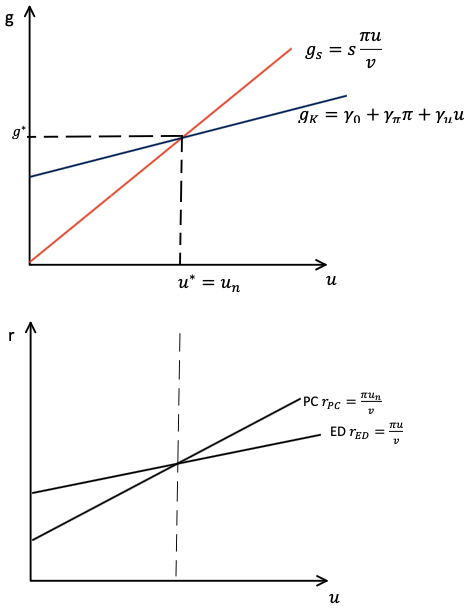
\includegraphics[width=1\linewidth,height=\textheight,keepaspectratio]{figuras/eqbm.png}

}

\caption{\label{fig-eqbm}Representação gráfica do modelo.}

\end{figure}%

A representação gráfica deste modelo, inicialmente, não se altera tanto
em relação à versão canônica do modelo.

De um lado, temos uma reta de crescimento da poupança positivamente
relacionada ao grau efetivo de utilização da capacidade instalada,
representando a Equação~\ref{eq-gs-bm}.

Por outro lado, a reta de investimento também responde positivamente ao
grau de utilização, além da distribuição de renda, conforme a
Equação~\ref{eq-gkbm}.

A interseção dessas duas curvas determina o equilíbrio simultâneo entre
crescimento e utilização da capacidade. O que pode ser imediatamente
transportado para o quadrante inferior da Figura~\ref{fig-eqbm}.

O que vemos na parte inferior é o encontro das curvas PC e ED,
representando a curva de Phillips e a de demanda efeitva
respectivamente. Enquanto a primeira (PC) é calculada com base no grau
desejado de utilização, onde as firmas atingem o \emph{markup} desejado,
a segunda registra a taxa de lucro efetivada a partir da demanda
realizada.

No equilíbrio, a dinâmica do grau de utilização garante a convergência
destas taxas de lucro \((r_{PC}=r_{ED}).\) Sempre que a poupança crescer
mais rápido que o investimento \((g_s>g_K)\), a taxa de lucro realizada
pelas firmas estará menor do que àquela que equilibraria o conflito
distributivo \((r_{ED}<r_{PC})\). Nestas circunstâncias, as firmas
deixarão de realizar novos investimentos, reduzindo o grau de utilização
em direção ao normal.

Sempre que o investimento crescer mais rápido que a poupança
\((g_K>g_s)\), o grau de utilização tende a se elevar. Com a demanda
efetiva gerando uma taxa de lucro realizada superior àquela que
equilibraria o conflito distributivo \((r_{ED}>r_{PC})\). A diferença
deste modelo reside no fato de que, agora, a parcela dos lucros na renda
influencia tanto a inclinação da taxa de crescimento da poupança (ver
Equação~\ref{eq-gs-bm}), quanto a taxa de crescimento do investimento
(ver Equação~\ref{eq-gkbm}). Portanto, alterações na distribuição de
renda terão efeito de:

\begin{itemize}
\item
  rotacionar a reta de crescimento da poupança \((g_s)\)
\item
  deslocar a reta de crescimento do investimento \((g_K)\)
\end{itemize}

\section{Paradoxo dos custos e da
parcimônia}\label{paradoxo-dos-custos-e-da-parcimuxf4nia}

Assim como discutido na \textbf{?@sec-paradoxos-kal}, temos que analisar
os paradoxos dos custos e da parcimônia (Thrifit) no fechamento
neo-kaleckiano.

\begin{tcolorbox}[enhanced jigsaw, arc=.35mm, bottomrule=.15mm, bottomtitle=1mm, breakable, colback=white, colbacktitle=quarto-callout-note-color!10!white, colframe=quarto-callout-note-color-frame, coltitle=black, left=2mm, leftrule=.75mm, opacityback=0, opacitybacktitle=0.6, rightrule=.15mm, title=\textcolor{quarto-callout-note-color}{\faInfo}\hspace{0.5em}{Lembrando os conceitos:}, titlerule=0mm, toprule=.15mm, toptitle=1mm]

Paradoxo dos custos \(\rightarrow\) sugere que o aumento dos salários,
ao aquecer a demanda efetiva, teria o resultado macroeconômico de elevar
a taxa de lucro das firmas.

\[\frac{\partial r}{\partial \pi} < 0 \]

Paradoxo da parcimônia \(\rightarrow\) sustenta que o aumento da
propensão marginal a poupar, ao desaquecer a demanda efetiva, teria
impacto negativo sobre a taxa de investimento e, portanto, sobre a
poupança macroecômica.

\[\begin{aligned}
\frac{\partial u}{\partial s} < 0\\ 
\& \\
\frac{\partial g}{\partial u} >0
\end{aligned}\]

\end{tcolorbox}

\begin{figure}[H]

{\centering 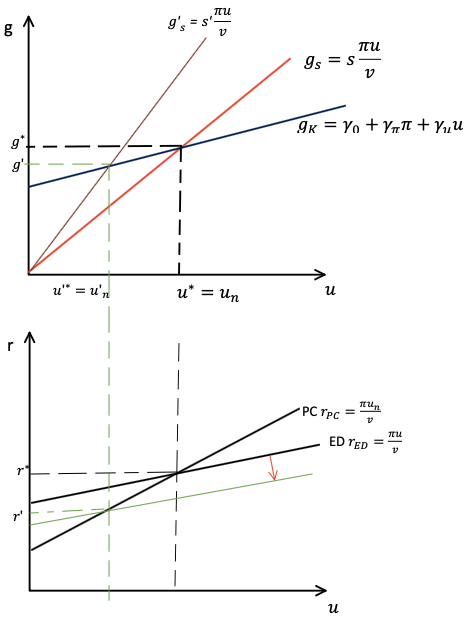
\includegraphics[width=1\linewidth,height=\textheight,keepaspectratio]{figuras/thrifitbm.png}

}

\caption{Parodoxo de Thrifit.}

\end{figure}%

O paradoxo de Thrifit segue válido no modelo neo-kaleckiano de Bhaduri e
Marglin.

Graficamente podemos constatar isso pela rotação que a mudança da
propensão a poupar causa na Equação~\ref{eq-gs-bm}. A curva \(g_s\)
rotaciona para dentro e intercepta a curva \(g_K\) em um novo ponto de
equilíbrio, com menores taxas de crescimento e de demanda.

Intuitivamente, temos que o aumento da propensão a poupar derruba o
consumo e reduz a demanda efetiva o que, para um dado \emph{markup}
desejado, faz com que as firmas optem por reduzir a taxa de crescimento
dos investimentos e manter sua parcela dos lucros na renda, ainda que
com menor taxa de lucro.

\[ s_\pi\downarrow \rightarrow g_s\downarrow \rightarrow u\downarrow \rightarrow g_K\downarrow \rightarrow u_n\downarrow \]

Algebricamente, não precisamos derivar para notar que o aumento de
\(s_\pi\) na Equação~\ref{eq-u-bm} leva ao aumento do denominador, fato
que reduz a razão. Ou seja, elevar \(s_\pi\) reduz \(u^*\).
Concomintantemente, pela Equação~\ref{eq-gkbm} vemos que a queda de
\(u\), tudo o mais constante, leva à queda de \(g_K\).

Assim, as duas condições para que o paradoxo de Thrifit ocorra foram
satisfeitas.

Já o paradoxo dos custos passa a ter um resultado ambíguo nesta versão
do modelo. Graficamente, vemos dois movimentos simultâneos:

\begin{itemize}
\item
  deslocamento da reta da taxa de investimentos \((g_K)\)
\item
  rotação da reta da taxa de poupança \((g_s)\)
\end{itemize}

\begin{figure}

\centering{

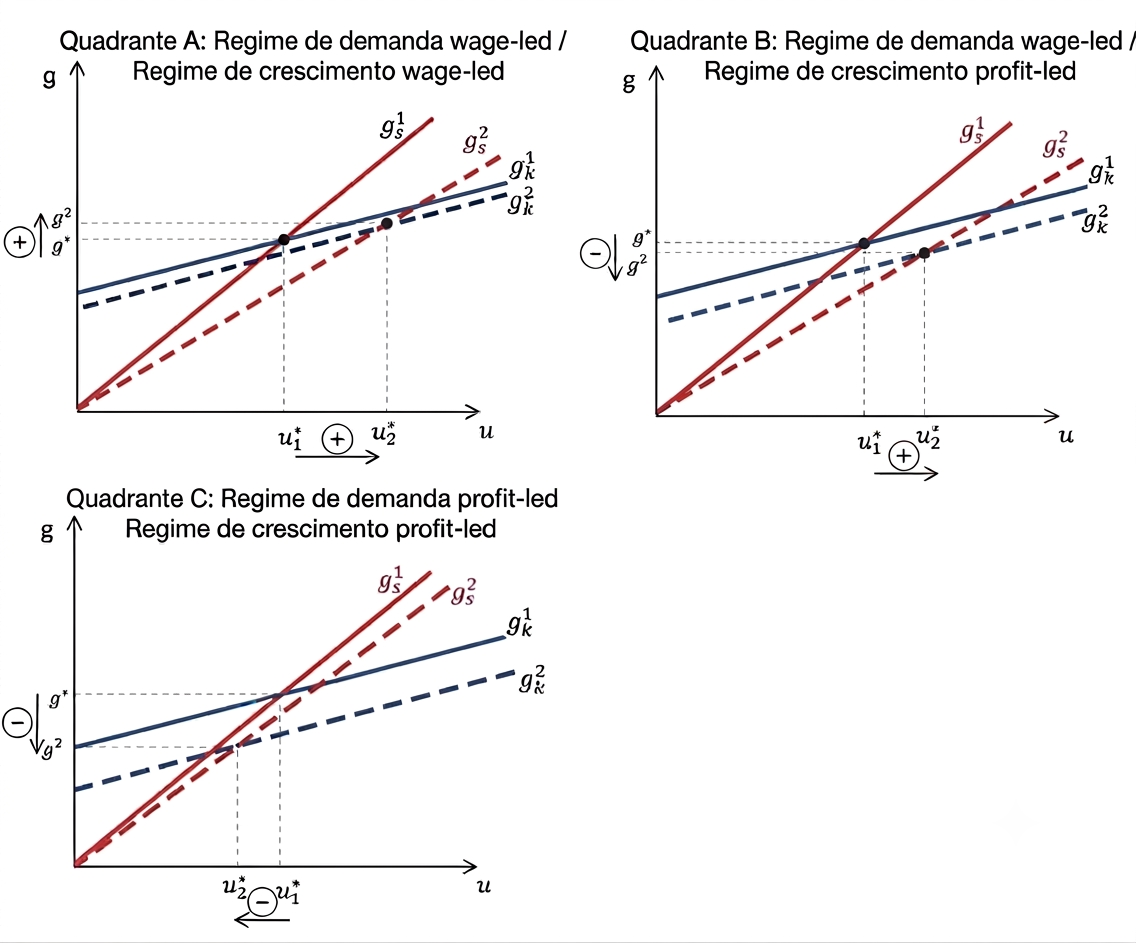
\includegraphics[width=1\linewidth,height=\textheight,keepaspectratio]{figuras/regimesbm.png}

}

\caption{\label{fig-custos-bm}Parodoxo dos custos}

\end{figure}%

A Figura~\ref{fig-custos-bm} ilustra o efeito de um aumento da parcela
dos salários na renda em três casos distintos. Se lembramos da
Equação~\ref{eq-r}, é fácil notar que para a taxa de lucro subir após o
aumento dos salários (queda da parcela dos lucros), é preciso que o grau
de utilização suba mais que proporcionalmente. Em outras palavras, o
paradoxo dos custos só será verificado em um regime de demanda
\emph{wage-led}. A seguir, vamos estudar esta relação entre parcela dos
salários na renda e grau de utilização.

Como trata-se de um gráfico bidimensional, que considera \(u\) e \(g\),
podemos pensar na mudança de \(\pi\) na Equação~\ref{eq-gkbm} como uma
mudança de intercepto da reta \(g_K\). Neste caso, o aumento dos
salários é equivalente à queda da parcela dos lucros, portanto,
diminuição do intercepto e, por isso, vemos um deslocamento para baixo
da reta \(g_K\).

Concomitantemente, ao olhar para Equação~\ref{eq-gs-bm} como uma equação
linear, podemos notar que o \(\pi\) funciona como um coeficiente angular
da reta. Ou seja, a queda do \(\pi\) reduz o coeficiente angular de uma
função de primeiro grau, reduzindo sua inclinação (rotacionando no
sentido horário). Em outras palavras: tornado a reta do plano cartesiano
mais ``deitada''.

O Quadrante A mostra que após a rotação da curva \(g_S\) no sentido
horário e o deslocamento para baixo de \(g_K\), o novo equilíbrio se dá
em um ponto compatível com maior grau de utilização e maior taxa de
crescimento. Enquanto o primeiro resultado denota um regime de demanda
liderado por salários, o segundo deve ser lido como um regime de
crescimento liderado pelos salários.

Em uma economia totalmente \emph{wage-led}, o conflito distributivo fica
menos intenso, já que o aumento dos salários leva ao aumento do ritmo de
acumulação do capital. Neste caso, o paradoxo dos custos pode ser
verificado no curto e no longo-prazo.

\begin{tcolorbox}[enhanced jigsaw, arc=.35mm, bottomrule=.15mm, bottomtitle=1mm, breakable, colback=white, colbacktitle=quarto-callout-warning-color!10!white, colframe=quarto-callout-warning-color-frame, coltitle=black, left=2mm, leftrule=.75mm, opacityback=0, opacitybacktitle=0.6, rightrule=.15mm, title=\textcolor{quarto-callout-warning-color}{\faExclamationTriangle}\hspace{0.5em}{Atenção}, titlerule=0mm, toprule=.15mm, toptitle=1mm]

Observe que o resultado do \textbf{Quadrante A} depende de um
deslocamento relativamente pequeno da curva \(g_K\) e de uma rotação
mais acentuada da curva \(g_S\).

Em termos econômicos, isso significa que o aumento da participação dos
salários na renda exerce apenas um efeito limitado sobre as expectativas
de lucratividade dos empresários, enquanto o estímulo ao consumo e à
demanda efetiva é suficientemente forte para elevar o grau de utilização
da capacidade instalada. Nessas circunstâncias, o efeito acelerador
sobre o investimento supera o efeito lucratividade, permitindo a
ocorrência de um regime de demanda e crescimento liderado pelos salários
(\emph{wage-led}).

\end{tcolorbox}

Como podemos notar pela Equação~\ref{eq-gkbm}, o tamanho do deslocamento
da curva de investimentos dependerá diretamente do quão sensível o
investimento é em relação à distribuição de renda (representado pelo
parâmero \(\gamma_\pi\)). Quanto mais sensível for, maior será o
deslocamento da reta \(g_K\), aumemtando as chances de um regime de
demanda profit-led (para dado \(\gamma_u\)).

Em suma e simplificadamente, o efeito líquido de uma distribuição de
renda em favor dos salários dependerá do efeito líquido entre o efeito
lucratividade \((\gamma_\pi)\) e o efeito acelerador \((\gamma_u)\).
Quanto maior for o efeito acelerador em relação ao efeito lucratividade,
maiores serão as chances de termos um regime de demanda e crescimento
liderado pelos salários (\emph{wage-led}).

O Quadrante B da Figura~\ref{fig-custos-bm} representa um modelo de
demanda wage-led, mas um regime de crescimento profit-led. Isto porque,
apesar de o grau de utilização crescer após o aumento da parcela dos
salários, isso não é suficiente para compensar a desaceleração do
investimento puxada pela consequente queda da parcela dos lucros.

Neste caso, a validade do paradoxo dos custos dependerá de o aumento do
grau de utilização compensar a queda da parcela dos lucros na renda, a
ponto de aumentar a taxa de lucro. Mais uma vez, menores serão as
chances disso acontecer, quanto maior for o efeito lucratividade do
investimento, capturado pelo parâmetro \(\gamma_\pi\). Aqui vemos como
um regime de demanda liderado pelos salários é condição necessária, mas
não suficiente para assegurar que o regime de crescimento também seja
liderado pelos salários (como vimos na Tabela~\ref{tbl-regimes}).

Por fim, o Quadrante C da Figura~\ref{fig-custos-bm} mostra que após o
aumento da parcela dos salários, o novo equilíbrio ocorre já com o grau
de utilização menor do que o inicial, caracterizando o regime de demanda
como liderado pelos lucros (\emph{profit-led}). Nestas circunstância,
não tem como o regime de crescimento não ser liderado pelos lucros
também, já que o efeito sensibilidade do investimento se mostrou
significativo ante o efeito acelerador, provocando um forte deslocamento
da curva \(g_K\). O paradoxo dos custos não é válido neste contexto.

Trabalhos empíricos conduzidos por autores neokaleckianos tendem a
mostrar um efeito acelerador bem alto, enquanto estimações apontam para
um baixo efeito lucratividade. Isto é, o investimento parece ser mais
sensível à demanda do que à lucratividade.

Intuitivamente, esta combinação de parâmetros, verificados
empiricamente, aumenta o efeito expansionista causado pela distribuição
de renda e minimiza o efeito contracionista causado pelo desestímulo ao
investimento devido a esta mesma distribuição.

\section{Seção de estudo interativo}\label{sec-estudo}

O gráfico abaixo permite explorar, de forma interativa, os efeitos de
alterações na propensão a poupar e na distribuição funcional da renda
sobre o equilíbrio do modelo neokaleckiano de Bhaduri e Marglin. Utilize
os controles deslizantes para modificar os parâmetros e observe como as
curvas e o ponto de equilíbrio se alteram.

\begin{tcolorbox}[enhanced jigsaw, arc=.35mm, bottomrule=.15mm, bottomtitle=1mm, breakable, colback=white, colbacktitle=quarto-callout-tip-color!10!white, colframe=quarto-callout-tip-color-frame, coltitle=black, left=2mm, leftrule=.75mm, opacityback=0, opacitybacktitle=0.6, rightrule=.15mm, title=\textcolor{quarto-callout-tip-color}{\faLightbulb}\hspace{0.5em}{Como utilizar o simulador}, titlerule=0mm, toprule=.15mm, toptitle=1mm]

\textbf{Paradoxo da parcimônia}

\begin{itemize}
\tightlist
\item
  Altere o \emph{slider} vermelho correspondente à propensão a poupar
  (\(s\)).
\item
  Observe a rotação da curva de poupança (\(g_S\)).
\item
  Compare a posição inicial (linha contínua) com a posição final (linha
  tracejada).
\end{itemize}

\textbf{Paradoxo dos custos}

\begin{itemize}
\tightlist
\item
  Altere o \emph{slider} verde correspondente à participação dos
  salários (\(w\)).
\item
  Observe simultaneamente:

  \begin{itemize}
  \tightlist
  \item
    a alteração da inclinação da curva de poupança;
  \item
    o deslocamento da curva de investimento, dada pela
    Equação~\ref{eq-gkbm};
  \item
    o novo ponto de equilíbrio.
  \end{itemize}
\end{itemize}

\end{tcolorbox}

\begin{tcolorbox}[enhanced jigsaw, arc=.35mm, bottomrule=.15mm, bottomtitle=1mm, breakable, colback=white, colbacktitle=quarto-callout-important-color!10!white, colframe=quarto-callout-important-color-frame, coltitle=black, left=2mm, leftrule=.75mm, opacityback=0, opacitybacktitle=0.6, rightrule=.15mm, title=\textcolor{quarto-callout-important-color}{\faExclamation}\hspace{0.5em}{O que observar?}, titlerule=0mm, toprule=.15mm, toptitle=1mm]

Durante a utilização do simulador, procure responder às seguintes
questões:

\begin{itemize}
\tightlist
\item
  Quais curvas se alteram quando aumenta a propensão a poupar (olhe o
  gráfico inferior também)?
\item
  O aumento da participação dos salários desloca ou rotaciona as curvas?
\item
  O que determina os regimes de demanda e de crescimento do modelo?
\end{itemize}

\end{tcolorbox}

\begin{tcolorbox}[enhanced jigsaw, arc=.35mm, bottomrule=.15mm, breakable, colback=white, colframe=quarto-callout-important-color-frame, left=2mm, leftrule=.75mm, opacityback=0, rightrule=.15mm, toprule=.15mm]

\end{tcolorbox}

\begin{tcolorbox}[enhanced jigsaw, arc=.35mm, bottomrule=.15mm, bottomtitle=1mm, breakable, colback=white, colbacktitle=quarto-callout-note-color!10!white, colframe=quarto-callout-note-color-frame, coltitle=black, left=2mm, leftrule=.75mm, opacityback=0, opacitybacktitle=0.6, rightrule=.15mm, title=\textcolor{quarto-callout-note-color}{\faInfo}\hspace{0.5em}{Exercício}, titlerule=0mm, toprule=.15mm, toptitle=1mm]

Após explorar diferentes valores para \(s\) e \(w\), explique, com suas
próprias palavras, os mecanismos econômicos responsáveis pelas
alterações observadas.

Sua resposta deve apresentar uma sequência lógica de causalidade,
identificando:

\begin{enumerate}
\def\labelenumi{\arabic{enumi}.}
\tightlist
\item
  qual parâmetro foi alterado;
\item
  quais curvas foram modificadas;
\item
  por que essas curvas se deslocaram ou rotacionaram;
\item
  como essas alterações afetaram o grau de utilização da capacidade e a
  taxa de crescimento;
\item
  Qual é o regime de demanda e de crescimento em cada caso.
\end{enumerate}

Evite apenas descrever o gráfico. Procure trazer a intuição econômica
representada pelo modelo.

\end{tcolorbox}

Agora, refaça o exercício anterior considerando o contexto do modelo
abaixo. A diferença entre os dois modelos são apenas os parâmteros
\(\gamma_\pi\) e \(\gamma_u\). Na versão abaixo, o investimento se
mostra muito mais sensível à mudanças da distribuição de renda e a taxa
de poupança menos sensível a esta mesma variável.

Repare que o regime de demanda e de crescimento não são o mesmo neste
contexto. Faça o exercício e tente identificar as principais
características presentes nesta representação. Explore os dois paradoxos
para aplicar o conhecimento construído ao longo deste capítulo.




\end{document}
